%%%%%%%%%%%%%%%%%%%%%%%%%%%%%%%%%%%%%%%%%
% Academic Paper Response Letter. 
% LaTeX Template
% Version 1.0 (20/07/2023)
% 
% This template refers to the toolbox tutorial (in Chinese):
% https://liam.page/2016/07/22/using-the-tcolorbox-package-to-create-a-new-theorem-environment/
% Please refer to the tutorial for your customization. 
% 
% Template license: Creative Commons CC BY 4.0
%
% Author: Yuhan Xie
% Contact email: yhxie0107@gmail.com
% Any revision advice is welcome!
% 
%%%%%%%%%%%%%%%%%%%%%%%%%%%%%%%%%%%%%%%%%


\documentclass{article}
%% Language and font encodings
%fixes to the latex2e kernel
%\usepackage{fixltx2e} %this is not needed after 2015
\usepackage{fix-cm}
\usepackage{etex}

%fix double floats numbering and positioning
\usepackage{dblfloatfix}

%checks for obsolete packages
\usepackage{nag}


%%% Local Variables: 
%%% mode: latex
%%% End: 

%Note: pagination needs to be loaded after graphics, because mdframed
%needs to be loaded after xcolor to keeep the our options for the latter
%colors
\makeatletter
\@ifpackageloaded{xcolor}{}{%
\usepackage[table,x11names,dvipsnames,svgnames]{xcolor}%
}
\makeatother

%colors in table
\usepackage{colortbl}

%pdf
\usepackage{graphicx}
\usepackage{wrapfig}

% Lyft colors (see https://design.lyft.com/re-approaching-color-9e604ba22c88)
\input{preamble/graphicsColors}

%%% Local Variables: 
%%% mode: latex
%%% End: 

\usepackage{cite}

%advanced typesetting
\usepackage{microtype}

%extensions for tables
\usepackage{array}
\usepackage{multirow}
\usepackage{booktabs}
\usepackage{makecell} %introduces \thead and \makecell

%compact paragraph title
\newcommand{\myparagraph}[1]{\textbf{\emph{#1}}.}
%\newcommand{\subparagraph}[1]{\emph{#1}.}

%provide options for changing spacing in enumeration environments
\ifcsname labelindent\endcsname
\let\labelindent\relax
\fi
\usepackage[inline]{enumitem}

%provides subfloats (subcaption replaces subfig and subfigure, but
%might not be compatible with some classes)
\usepackage{subfig}

\providecommand{\ie}{i.e.}
\providecommand{\eg}{e.g.}
\providecommand{\etal}{et al.}

%set more relaxed constraints on the floats
\setcounter{topnumber}{2}
\setcounter{bottomnumber}{2}
\setcounter{totalnumber}{4}
\renewcommand{\topfraction}{0.85}
\renewcommand{\bottomfraction}{0.85}
\renewcommand{\textfraction}{0.15}
\renewcommand{\floatpagefraction}{0.7}

%Make an enumeration with a letter+progressive number
\newenvironment{lenumerate}[2][]
{\begin{enumerate}[label=(#2\arabic*),leftmargin=0.2in,itemindent=0.15in,#1]}
{\end{enumerate}}

%Make an letter+progressive number description list
\newenvironment{ldescription}[2][]
{\begin{lenumerate}{#2}%
\let\bitem\item%
\renewcommand{\item}[1][]{\bitem\textsl{##1}:~}}
{\end{lenumerate}}


 %The following sets the labeling for inline enumerations

\setlist*[enumerate,1]{label={\itshape\arabic*)}}

%Define macro to make paragraph headings always end with a full stop
\makeatletter
\newcommand{\paragraphswithstop}{%
\let\copyparagraph\paragraph%
\renewcommand\paragraph[1]{\copyparagraph{##1.}}%
}
\makeatother

%Package to frame text in boxes
\usepackage[framemethod=tikz]{mdframed}

%%% Local Variables: 
%%% mode: latex
%%% End: 

%
% Allow easy definition of starred version of commands
% Ref: https://tex.stackexchange.com/questions/202504/macro-to-add-starred-version-of-command
\usepackage{suffix}

% Allow definition of environments with extra final code
\usepackage{environ}

% Insert a prefix-argument-postfix text only if argument is non-empty
% Needs to use a savebox to avoid evaluating the argument multiple times
\makeatletter
\newsavebox{\boxifnotempty}
\newcommand{\displayifnotempty}[3]{\sbox\boxifnotempty{#2}\setbox0=\hbox{\usebox{\boxifnotempty}\unskip}%
\ifdim\wd0=0pt
\else
 #1\usebox{\boxifnotempty}#3%
\fi%
}
\newcommand{\ifempty}[2]{\setbox0=\hbox{#1\unskip}%
\ifdim\wd0=0pt%
 #2%
\fi%
}
\newcommand{\ifnotempty}[2]{\setbox0=\hbox{#1\unskip}%
\ifdim\wd0>0pt%
 #2%
\fi%
}
\makeatother

%introduce the algorithmic environment and the algorithm floats
\usepackage{algpseudocode}
\usepackage{algorithm}

%macros for storing definitions across compilations
\usepackage{scrlfile}

\makeatletter
%mark a definition to be stored in the aux file
\newcommand*\newstoreddef[1]{
  \BeforeClosingMainAux{%
    \immediate\write\@auxout{%
      \string\restoredef{#1}{\csname #1\endcsname}%
    }%
  }%
}
%used by the aux file to restore the definition
\newcommand*{\restoredef}[2]{% used at the aux file
  \expandafter\gdef\csname stored@#1\endcsname{#2}%
}
%show the stored definition (user command to ask for the value)
\newcommand*{\storeddef}[1]{
  \@ifundefined{stored@#1}{0}{\csname stored@#1\endcsname}%
}
\makeatother

%Add values to non-counter definitions (works with non-integers)
\newcommand{\addtovar}[2]{\pgfmathparse{#1+#2}\xdef#1{\pgfmathresult}}
\newcommand{\zerovar}[1]{\xdef#1{0}}

%Insert content of a PGF variable 
\newcommand{\pgfprint}[1]{\pgfmathparse{#1}\pgfmathresult}

%Package to get PDF page numbers
\usepackage{pageslts}
%\pagenumbering{arabic}
%Output content of enviroment both to the document and to the log file
%In the log file, the content is marked by start/end delimiters, and
%macros are not expanded.
\NewEnviron{tee}{\BODY\typeout{Marker Tee [start] ^^J \BODY ^^JMaker Tee [end]}}


%%% Local Variables: 
%%% mode: latex
%%% End: 

%AMS typesetting
\makeatletter
\@ifpackageloaded{amsmath}{}{%
\usepackage[cmex10]{amsmath}%
}
\makeatother
\usepackage{mathtools}
\usepackage{amssymb,amsfonts}
\makeatletter
\@ifundefined{proof}{%
\usepackage{amsthm}%
}{}
\makeatother

\usepackage{mathtools}

%Common math statements environments
\makeatletter
\@ifundefined{theorem}{
\newtheorem{theorem}{Theorem}
\newtheorem{corollary}{Corollary}
\newtheorem{proposition}{Proposition}
\newtheorem{lemma}{Lemma}
\newtheorem{remark}{Remark}
\newtheorem{fact}{Fact}
}{}
  %SIAM article classes give their own Definition and Remark environments
\@ifundefined{definition}{
  \newtheorem{definition}{Definition}
}
% \@ifundefined{remark}{
%   \newtheorem{remark}{Remark}
% }
\makeatother
\newtheorem{problem}{Problem}
\newtheorem{assumption}{Assumption}
\newtheorem{property}{Property}
\newcommand{\rmss}[1]{_{\textrm{#1}}}

%%% Local Variables: 
%%% mode: latex
%%% End: 

%Spaces
\newcommand{\real}[1]{\mathbb{R}^{#1}{}}
\newcommand{\complex}[1]{\mathbb{C}^{#1}{}}
\newcommand{\naturals}[1]{\mathbb{N}^{#1}{}}
\newcommand{\integers}[1]{\mathbb{Z}^{#1}{}}
\newcommand{\sphere}[1]{{\mathbb{S}^{#1}}{}}
\newcommand{\stiefel}{\mathrm{St}}
\newcommand{\grassmann}{\mathrm{Grass}}
\newcommand{\GL}{\mathbb{GL}}

%short-hand for matrices
\newcommand{\bmat}[1]{\begin{bmatrix}#1\end{bmatrix}}
\newcommand{\Bmat}[1]{\begin{Bmatrix}#1\end{Bmatrix}}
\newcommand{\pmat}[1]{\begin{pmatrix}#1\end{pmatrix}}

%supertscript operators
\newcommand{\transpose}{^\mathrm{T}}
\newcommand{\hermitian}{^\mathrm{H}}
\newcommand{\inverse}{^{-1}}
\newcommand{\pinverse}{^\dagger}
\newcommand{\orth}{^{\bot}}
\newcommand{\apstar}{^{\ast}}

%parentheses-based operators
\newcommand{\cross}[1]{[#1]_{\times}\!}
\newcommand{\crossinv}[1]{[#1]_{\times}^{\textrm{inv}}\!}

%equality
\newcommand{\defeq}{\doteq}


%Norms, absolute values, and inner products
\DeclarePairedDelimiter{\abs}{\lvert}{\rvert}
\DeclarePairedDelimiter{\ceil}{\lceil}{\rceil}
\DeclarePairedDelimiter{\norm}{\lVert}{\rVert}
\newcommand{\frob}[1]{\norm{#1}_F}
\newcommand{\bigfrob}[1]{\bignorm{#1}_F}
\newcommand{\metric}[3][]{g_{#1}\left(#2, #3\right)}
\newcommand{\metrica}[3]{\langle #2, #3\rangle_{#1}}

%Derivatives
\newcommand{\de}{\mathrm{d}}
\newcommand{\dert}[1][]{\frac{\de #1}{\de t}}
\newcommand{\ddert}[1][]{\frac{\de^2 #1}{\de t^2}}
%Vector
\newcommand{\vct}[1]{\mathbf{#1}}
\newcommand{\pder}[2][]{\frac{\partial #1}{\partial #2}}
%named operators
\DeclareMathOperator*{\Land}{\bigwedge}
\DeclareMathOperator{\rank}{rank}
\DeclareMathOperator{\diag}{diag}
\DeclareMathOperator{\blkdiag}{blkdiag}
\DeclareMathOperator{\symm}{sym}
\DeclareMathOperator{\asym}{skew}
\DeclareMathOperator*{\argmin}{\arg\!\min}
\DeclareMathOperator{\softmin}{softmin}
\DeclareMathOperator*{\argmax}{\arg\!\max}
\DeclareMathOperator{\trace}{tr}
\DeclareMathOperator{\vecspan}{span}
\DeclareMathOperator{\vecnull}{null}
\DeclareMathOperator{\vecnullity}{nullity}
\DeclareMathOperator{\vecop}{vec}
\DeclareMathOperator{\stack}{stack}
\DeclareMathOperator{\hstack}{hstack}
\DeclareMathOperator{\vstack}{vstack}
\DeclareMathOperator{\sign}{sign}
\DeclareMathOperator{\sinc}{sinc}
\DeclareMathOperator{\expm}{expm}

\DeclareMathOperator{\grad}{{grad}}
\DeclareMathOperator{\D}{D\!}
\DeclareMathOperator{\Dgrad}{{Dgrad}}
\DeclareMathOperator{\hess}{{Hess}}

\DeclareMathOperator*{\inj}{inj}
\DeclareMathOperator{\hull}{hull}

\DeclareMathOperator{\proj}{{proj}}

\DeclareMathOperator*{\logm}{logm}
\DeclareMathOperator{\Log}{Log}
\DeclareMathOperator{\LogNorm}{\frac{Log}{\norm{Log}}}
\DeclareMathOperator{\DLog}{DLog}
\DeclareMathOperator{\DLogNorm}{D\frac{Log}{\norm{Log}}}

\DeclareMathOperator{\conv}{conv}
\DeclareMathOperator{\cvxhull}{co}

\DeclareMathOperator{\dist}{dist}

\DeclareMathOperator*{\bigO}{O}

%\DeclareMathOperator*{\Pr}
\newcommand{\intersect}{\cap}
\newcommand{\union}{\cup}
\DeclareMathOperator*{\Or}{\bigvee}

%text for constrained optimization
\newcommand{\subjectto}{\textrm{subject to }}

%%% Local Variables: 
%%% mode: latex
%%% End: 


%memberships
\newcommand{\iV}[1][]{{i \in V_{#1}}}
\newcommand{\ijE}[1][]{(i,j) \in E_{#1}}

%operators
\DeclareMathOperator{\dg}{{deg}}
\DeclareMathOperator{\diam}{{Diam}}

%%% Local Variables: 
%%% mode: latex
%%% End: 

% This file was generated by the scriptgenerateNotation
% Do not modify this file directly

% Shortand notation for vectors and their derivatives
\providecommand{\va}{\vct{a}}
\providecommand{\dva}{\dot{\vct{a}}}
\providecommand{\tva}{\tilde{\vct{a}}}
\providecommand{\dtva}{\dot{\tilde{\vct{a}}}}
\providecommand{\vb}{\vct{b}}
\providecommand{\dvb}{\dot{\vct{b}}}
\providecommand{\tvb}{\tilde{\vct{b}}}
\providecommand{\dtvb}{\dot{\tilde{\vct{b}}}}
\providecommand{\vc}{\vct{c}}
\providecommand{\dvc}{\dot{\vct{c}}}
\providecommand{\tvc}{\tilde{\vct{c}}}
\providecommand{\dtvc}{\dot{\tilde{\vct{c}}}}
\providecommand{\vd}{\vct{d}}
\providecommand{\dvd}{\dot{\vct{d}}}
\providecommand{\tvd}{\tilde{\vct{d}}}
\providecommand{\dtvd}{\dot{\tilde{\vct{d}}}}
\providecommand{\ve}{\vct{e}}
\providecommand{\dve}{\dot{\vct{e}}}
\providecommand{\tve}{\tilde{\vct{e}}}
\providecommand{\dtve}{\dot{\tilde{\vct{e}}}}
\providecommand{\vf}{\vct{f}}
\providecommand{\dvf}{\dot{\vct{f}}}
\providecommand{\tvf}{\tilde{\vct{f}}}
\providecommand{\dtvf}{\dot{\tilde{\vct{f}}}}
\providecommand{\vg}{\vct{g}}
\providecommand{\dvg}{\dot{\vct{g}}}
\providecommand{\tvg}{\tilde{\vct{g}}}
\providecommand{\dtvg}{\dot{\tilde{\vct{g}}}}
\providecommand{\vh}{\vct{h}}
\providecommand{\dvh}{\dot{\vct{h}}}
\providecommand{\tvh}{\tilde{\vct{h}}}
\providecommand{\dtvh}{\dot{\tilde{\vct{h}}}}
\providecommand{\vi}{\vct{i}}
\providecommand{\dvi}{\dot{\vct{i}}}
\providecommand{\tvi}{\tilde{\vct{i}}}
\providecommand{\dtvi}{\dot{\tilde{\vct{i}}}}
\providecommand{\vj}{\vct{j}}
\providecommand{\dvj}{\dot{\vct{j}}}
\providecommand{\tvj}{\tilde{\vct{j}}}
\providecommand{\dtvj}{\dot{\tilde{\vct{j}}}}
\providecommand{\vk}{\vct{k}}
\providecommand{\dvk}{\dot{\vct{k}}}
\providecommand{\tvk}{\tilde{\vct{k}}}
\providecommand{\dtvk}{\dot{\tilde{\vct{k}}}}
\providecommand{\vl}{\vct{l}}
\providecommand{\dvl}{\dot{\vct{l}}}
\providecommand{\tvl}{\tilde{\vct{l}}}
\providecommand{\dtvl}{\dot{\tilde{\vct{l}}}}
\providecommand{\vm}{\vct{m}}
\providecommand{\dvm}{\dot{\vct{m}}}
\providecommand{\tvm}{\tilde{\vct{m}}}
\providecommand{\dtvm}{\dot{\tilde{\vct{m}}}}
\providecommand{\vn}{\vct{n}}
\providecommand{\dvn}{\dot{\vct{n}}}
\providecommand{\tvn}{\tilde{\vct{n}}}
\providecommand{\dtvn}{\dot{\tilde{\vct{n}}}}
\providecommand{\vo}{\vct{o}}
\providecommand{\dvo}{\dot{\vct{o}}}
\providecommand{\tvo}{\tilde{\vct{o}}}
\providecommand{\dtvo}{\dot{\tilde{\vct{o}}}}
\providecommand{\vp}{\vct{p}}
\providecommand{\dvp}{\dot{\vct{p}}}
\providecommand{\tvp}{\tilde{\vct{p}}}
\providecommand{\dtvp}{\dot{\tilde{\vct{p}}}}
\providecommand{\vq}{\vct{q}}
\providecommand{\dvq}{\dot{\vct{q}}}
\providecommand{\tvq}{\tilde{\vct{q}}}
\providecommand{\dtvq}{\dot{\tilde{\vct{q}}}}
\providecommand{\vr}{\vct{r}}
\providecommand{\dvr}{\dot{\vct{r}}}
\providecommand{\tvr}{\tilde{\vct{r}}}
\providecommand{\dtvr}{\dot{\tilde{\vct{r}}}}
\providecommand{\vs}{\vct{s}}
\providecommand{\dvs}{\dot{\vct{s}}}
\providecommand{\tvs}{\tilde{\vct{s}}}
\providecommand{\dtvs}{\dot{\tilde{\vct{s}}}}
\providecommand{\vt}{\vct{t}}
\providecommand{\dvt}{\dot{\vct{t}}}
\providecommand{\tvt}{\tilde{\vct{t}}}
\providecommand{\dtvt}{\dot{\tilde{\vct{t}}}}
\providecommand{\vu}{\vct{u}}
\providecommand{\dvu}{\dot{\vct{u}}}
\providecommand{\tvu}{\tilde{\vct{u}}}
\providecommand{\dtvu}{\dot{\tilde{\vct{u}}}}
\providecommand{\vv}{\vct{v}}
\providecommand{\dvv}{\dot{\vct{v}}}
\providecommand{\tvv}{\tilde{\vct{v}}}
\providecommand{\dtvv}{\dot{\tilde{\vct{v}}}}
\providecommand{\vw}{\vct{w}}
\providecommand{\dvw}{\dot{\vct{w}}}
\providecommand{\tvw}{\tilde{\vct{w}}}
\providecommand{\dtvw}{\dot{\tilde{\vct{w}}}}
\providecommand{\vx}{\vct{x}}
\providecommand{\dvx}{\dot{\vct{x}}}
\providecommand{\tvx}{\tilde{\vct{x}}}
\providecommand{\dtvx}{\dot{\tilde{\vct{x}}}}
\providecommand{\vy}{\vct{y}}
\providecommand{\dvy}{\dot{\vct{y}}}
\providecommand{\tvy}{\tilde{\vct{y}}}
\providecommand{\dtvy}{\dot{\tilde{\vct{y}}}}
\providecommand{\vz}{\vct{z}}
\providecommand{\dvz}{\dot{\vct{z}}}
\providecommand{\tvz}{\tilde{\vct{z}}}
\providecommand{\dtvz}{\dot{\tilde{\vct{z}}}}
\providecommand{\vA}{\vct{A}}
\providecommand{\dvA}{\dot{\vct{A}}}
\providecommand{\tvA}{\tilde{\vct{A}}}
\providecommand{\dtvA}{\dot{\tilde{\vct{A}}}}
\providecommand{\vB}{\vct{B}}
\providecommand{\dvB}{\dot{\vct{B}}}
\providecommand{\tvB}{\tilde{\vct{B}}}
\providecommand{\dtvB}{\dot{\tilde{\vct{B}}}}
\providecommand{\vC}{\vct{C}}
\providecommand{\dvC}{\dot{\vct{C}}}
\providecommand{\tvC}{\tilde{\vct{C}}}
\providecommand{\dtvC}{\dot{\tilde{\vct{C}}}}
\providecommand{\vD}{\vct{D}}
\providecommand{\dvD}{\dot{\vct{D}}}
\providecommand{\tvD}{\tilde{\vct{D}}}
\providecommand{\dtvD}{\dot{\tilde{\vct{D}}}}
\providecommand{\vE}{\vct{E}}
\providecommand{\dvE}{\dot{\vct{E}}}
\providecommand{\tvE}{\tilde{\vct{E}}}
\providecommand{\dtvE}{\dot{\tilde{\vct{E}}}}
\providecommand{\vF}{\vct{F}}
\providecommand{\dvF}{\dot{\vct{F}}}
\providecommand{\tvF}{\tilde{\vct{F}}}
\providecommand{\dtvF}{\dot{\tilde{\vct{F}}}}
\providecommand{\vG}{\vct{G}}
\providecommand{\dvG}{\dot{\vct{G}}}
\providecommand{\tvG}{\tilde{\vct{G}}}
\providecommand{\dtvG}{\dot{\tilde{\vct{G}}}}
\providecommand{\vH}{\vct{H}}
\providecommand{\dvH}{\dot{\vct{H}}}
\providecommand{\tvH}{\tilde{\vct{H}}}
\providecommand{\dtvH}{\dot{\tilde{\vct{H}}}}
\providecommand{\vI}{\vct{I}}
\providecommand{\dvI}{\dot{\vct{I}}}
\providecommand{\tvI}{\tilde{\vct{I}}}
\providecommand{\dtvI}{\dot{\tilde{\vct{I}}}}
\providecommand{\vJ}{\vct{J}}
\providecommand{\dvJ}{\dot{\vct{J}}}
\providecommand{\tvJ}{\tilde{\vct{J}}}
\providecommand{\dtvJ}{\dot{\tilde{\vct{J}}}}
\providecommand{\vK}{\vct{K}}
\providecommand{\dvK}{\dot{\vct{K}}}
\providecommand{\tvK}{\tilde{\vct{K}}}
\providecommand{\dtvK}{\dot{\tilde{\vct{K}}}}
\providecommand{\vL}{\vct{L}}
\providecommand{\dvL}{\dot{\vct{L}}}
\providecommand{\tvL}{\tilde{\vct{L}}}
\providecommand{\dtvL}{\dot{\tilde{\vct{L}}}}
\providecommand{\vM}{\vct{M}}
\providecommand{\dvM}{\dot{\vct{M}}}
\providecommand{\tvM}{\tilde{\vct{M}}}
\providecommand{\dtvM}{\dot{\tilde{\vct{M}}}}
\providecommand{\vN}{\vct{N}}
\providecommand{\dvN}{\dot{\vct{N}}}
\providecommand{\tvN}{\tilde{\vct{N}}}
\providecommand{\dtvN}{\dot{\tilde{\vct{N}}}}
\providecommand{\vO}{\vct{O}}
\providecommand{\dvO}{\dot{\vct{O}}}
\providecommand{\tvO}{\tilde{\vct{O}}}
\providecommand{\dtvO}{\dot{\tilde{\vct{O}}}}
\providecommand{\vP}{\vct{P}}
\providecommand{\dvP}{\dot{\vct{P}}}
\providecommand{\tvP}{\tilde{\vct{P}}}
\providecommand{\dtvP}{\dot{\tilde{\vct{P}}}}
\providecommand{\vQ}{\vct{Q}}
\providecommand{\dvQ}{\dot{\vct{Q}}}
\providecommand{\tvQ}{\tilde{\vct{Q}}}
\providecommand{\dtvQ}{\dot{\tilde{\vct{Q}}}}
\providecommand{\vR}{\vct{R}}
\providecommand{\dvR}{\dot{\vct{R}}}
\providecommand{\tvR}{\tilde{\vct{R}}}
\providecommand{\dtvR}{\dot{\tilde{\vct{R}}}}
\providecommand{\vS}{\vct{S}}
\providecommand{\dvS}{\dot{\vct{S}}}
\providecommand{\tvS}{\tilde{\vct{S}}}
\providecommand{\dtvS}{\dot{\tilde{\vct{S}}}}
\providecommand{\vT}{\vct{T}}
\providecommand{\dvT}{\dot{\vct{T}}}
\providecommand{\tvT}{\tilde{\vct{T}}}
\providecommand{\dtvT}{\dot{\tilde{\vct{T}}}}
\providecommand{\vU}{\vct{U}}
\providecommand{\dvU}{\dot{\vct{U}}}
\providecommand{\tvU}{\tilde{\vct{U}}}
\providecommand{\dtvU}{\dot{\tilde{\vct{U}}}}
\providecommand{\vV}{\vct{V}}
\providecommand{\dvV}{\dot{\vct{V}}}
\providecommand{\tvV}{\tilde{\vct{V}}}
\providecommand{\dtvV}{\dot{\tilde{\vct{V}}}}
\providecommand{\vW}{\vct{W}}
\providecommand{\dvW}{\dot{\vct{W}}}
\providecommand{\tvW}{\tilde{\vct{W}}}
\providecommand{\dtvW}{\dot{\tilde{\vct{W}}}}
\providecommand{\vX}{\vct{X}}
\providecommand{\dvX}{\dot{\vct{X}}}
\providecommand{\tvX}{\tilde{\vct{X}}}
\providecommand{\dtvX}{\dot{\tilde{\vct{X}}}}
\providecommand{\vY}{\vct{Y}}
\providecommand{\dvY}{\dot{\vct{Y}}}
\providecommand{\tvY}{\tilde{\vct{Y}}}
\providecommand{\dtvY}{\dot{\tilde{\vct{Y}}}}
\providecommand{\vZ}{\vct{Z}}
\providecommand{\dvZ}{\dot{\vct{Z}}}
\providecommand{\tvZ}{\tilde{\vct{Z}}}
\providecommand{\dtvZ}{\dot{\tilde{\vct{Z}}}}

\providecommand{\vbeta}{\boldsymbol{\beta}}
\providecommand{\dvbeta}{\dot{\boldsymbol{\beta}}}
\providecommand{\vsigma}{\boldsymbol{\sigma}}
\providecommand{\dvsigma}{\dot{\boldsymbol{\sigma}}}

% Shortand notation for derivatives and bold of symbols
\providecommand{\te}{\tilde{e}}

\providecommand{\dgamma}{\dot{\gamma}}
\providecommand{\ddgamma}{\ddot{\gamma}}
\providecommand{\vgamma}{\bm{\gamma}}
\providecommand{\dDelta}{\dot{\Delta}}
\providecommand{\ddDelta}{\ddot{\Delta}}
\providecommand{\vDelta}{\bm{\Delta}}

% Shortand notation for matrices
\providecommand{\mA}{\vct{A}}
\providecommand{\mB}{\vct{B}}
\providecommand{\mC}{\vct{C}}
\providecommand{\mD}{\vct{D}}
\providecommand{\mE}{\vct{E}}
\providecommand{\mF}{\vct{F}}
\providecommand{\mG}{\vct{G}}
\providecommand{\mH}{\vct{H}}
\providecommand{\mI}{\vct{I}}
\providecommand{\mJ}{\vct{J}}
\providecommand{\mK}{\vct{K}}
\providecommand{\mL}{\vct{L}}
\providecommand{\mM}{\vct{M}}
\providecommand{\mN}{\vct{N}}
\providecommand{\mO}{\vct{O}}
\providecommand{\mP}{\vct{P}}
\providecommand{\mQ}{\vct{Q}}
\providecommand{\mR}{\vct{R}}
\providecommand{\mS}{\vct{S}}
\providecommand{\mT}{\vct{T}}
\providecommand{\mU}{\vct{U}}
\providecommand{\mV}{\vct{V}}
\providecommand{\mW}{\vct{W}}
\providecommand{\mX}{\vct{X}}
\providecommand{\mY}{\vct{Y}}
\providecommand{\mZ}{\vct{Z}}

% Shortand notation for calligraphic upper case letters
\providecommand{\cA}{\mathcal{A}}
\providecommand{\cB}{\mathcal{B}}
\providecommand{\cC}{\mathcal{C}}
\providecommand{\cD}{\mathcal{D}}
\providecommand{\cE}{\mathcal{E}}
\providecommand{\cF}{\mathcal{F}}
\providecommand{\cG}{\mathcal{G}}
\providecommand{\cH}{\mathcal{H}}
\providecommand{\cI}{\mathcal{I}}
\providecommand{\cJ}{\mathcal{J}}
\providecommand{\cK}{\mathcal{K}}
\providecommand{\cL}{\mathcal{L}}
\providecommand{\cM}{\mathcal{M}}
\providecommand{\cN}{\mathcal{N}}
\providecommand{\cO}{\mathcal{O}}
\providecommand{\cP}{\mathcal{P}}
\providecommand{\cQ}{\mathcal{Q}}
\providecommand{\cR}{\mathcal{R}}
\providecommand{\cS}{\mathcal{S}}
\providecommand{\cT}{\mathcal{T}}
\providecommand{\cU}{\mathcal{U}}
\providecommand{\cV}{\mathcal{V}}
\providecommand{\cW}{\mathcal{W}}
\providecommand{\cX}{\mathcal{X}}
\providecommand{\cY}{\mathcal{Y}}
\providecommand{\cZ}{\mathcal{Z}}

% Shortand notation for some tilded symbols and their derivatives
\providecommand{\tx}{\tilde{x}}
\providecommand{\dtx}{\dot{\tilde{x}}}
\providecommand{\ty}{\tilde{y}}
\providecommand{\dty}{\dot{\tilde{y}}}
\providecommand{\tvarphi}{\tilde{\varphi}}
\providecommand{\dtvarphi}{\dot{\tilde{\varphi}}}

% Shrtand notation for Frame representation
\newcommand{\Fframe}[1]{{#1^{\cF}}}
\newcommand{\Eframe}[1]{{#1^{\cE}}}

% shortand notation for temporal logic
\newcommand{\TLand}{\vee}
\newcommand{\TLor}{\wedge}


%command for units of measure
\usepackage{units}

%S.I. units for some standard quantities
\newcommand{\upos}[1][]{\unit[#1]{m}}
\newcommand{\urad}[1][]{\unit[#1]{rad}}
\newcommand{\uvel}[1][]{\unitfrac[#1]{m}{s}}
\newcommand{\uacc}[1][]{\unitfrac[#1]{m}{s^2}}
\newcommand{\uavel}[1][]{\unitfrac[#1]{rad}{s}}
\newcommand{\uaacc}[1][]{\unitfrac[#1]{rad}{s^2}}
\newcommand{\uforce}[1][]{\unit[#1]{N}}
\newcommand{\utime}[1][]{\unit[#1]{s}}
\newcommand{\umass}[1][]{\unit[#1]{kg}}
\newcommand{\uspring}[1][]{\unitfrac[#1]{N}{m}}
\newcommand{\udamping}[1][]{\unitfrac[#1]{N\cdot s}{m}}
\newcommand{\ulength}[1][]{\unit[#1]{m}}
\newcommand{\uinertia}[1][]{\unit[#1]{kg\cdot m^2}}


%macro to define other macros for block-colored labels
\newcommand{\newcolorlabel}[2]{%
  \expandafter\newcommand\csname #1\endcsname[1]{%
    \colorbox{#2}{\color{white}\textsf{\textbf{##1}}}}%
}

%macro to define other macros for comments 
%
\newcommand{\newcommenter}[2]{%
  \expandafter\newcommand\csname #1\endcsname[1]{%
    \fcolorbox{#2}{#2}{\color{white}\textsf{\textbf{#1}}}
    {\color{#2}##1}}%
  %comment to mention commenter
  \expandafter\newcommand\csname at#1\endcsname{%
    \fcolorbox{#2}{#2}{\color{white}\textsf{\textbf{@#1}}}
    {\color{#2}}}%
  % comment to highlight
  \expandafter\newcommand\csname #1hl\endcsname[2]{%
    \colorbox{#2}{\color{white}\textsf{\textbf{#1}}}\sethlcolor{Azure2}\hl{##2}~%
    \expandafter\ifx\csname commentarrow\endcsname\relax$\leftarrow$\else \commentarrow[#2]\fi~%
    {\color{#2}##1}}%
  % comment to strikeout
  \expandafter\newcommand\csname #1st\endcsname[2]{%
    \colorbox{#2}{\color{white}\textsf{\textbf{#1}}}\sout{##2}~%
    \expandafter\ifx\csname commentarrow\endcsname\relax$\leftarrow$\else \commentarrow[#2]\fi~%
    {\color{#2}##1}}%
}
% examples of the macro above
\newcommenter{TODO}{DodgerBlue1}
\newcommenter{rtron}{Green3}
\newcommenter{zyang}{orange}
%side review pointer
\newcommand{\toreview}{\tikz[overlay, remember picture]{\coordinate (center); \node[fill=red] at (current page.center |- center){};}}

%introduce the comment environment
\usepackage{comment}

%enable pdf annotation
\usepackage{pdfcomment}

%enable highlights
\usepackage{soul}

%enable strikeout text with the command \sout{}
\usepackage[normalem]{ulem}

%package for displayed text
\usepackage{csquotes}

%markup
\newcommand{\file}[1]{\mbox{\texttt{#1}}}
\newcommand{\var}[1]{\mbox{\texttt{#1}}}

\newcommand{\function}[3][]{\displayifnotempty{[}{\var{#1}}{]=}\file{\mbox{#2}}(\var{#3})}

\newcommand{\key}[1]{\mbox{\textcolor{DodgerBlue3}{\texttt{#1}}}}

\newcommand{\displayfunction}[3][]{\begin{displayquote}\function[#1]{#2}{#3}\end{displayquote}}
\newcommand{\vardim}[2]{[\texttt{#1}~$\times$~\texttt{#2}]}


%%% Local Variables: 
%%% mode: latex
%%% End: 

%TikZ and common libraries
\usepackage{tikz}
\usetikzlibrary{calc}
\usetikzlibrary{matrix}
\usetikzlibrary{chains}
\usetikzlibrary{shapes.geometric}
\usetikzlibrary{arrows.meta}
\usetikzlibrary{decorations.pathreplacing}
\usetikzlibrary{backgrounds}

%Draw normalized vector between two coordinates
\newcommand\normalize[2][(0,0)]{%
  \draw[blue,->] (#1) -- ($(#1)!1cm!(#2)$) coordinate (#1#2norm)}

%Quotatures
\tikzset{
  dim above/.style={to path={\pgfextra{
        \pgfinterruptpath
        \draw[>=latex,|->|] let
        \p1=($(\tikztostart)!1.5em!90:(\tikztotarget)$),
        \p2=($(\tikztotarget)!1.5em!-90:(\tikztostart)$)
        in(\p1) -- (\p2) node[pos=.5,sloped,above]{#1};
        \endpgfinterruptpath
      }
    }
  },
  dim double above/.style={to path={\pgfextra{
        \pgfinterruptpath
        \draw[>=latex,|->|] let
        \p1=($(\tikztostart)!3em!90:(\tikztotarget)$),
        \p2=($(\tikztotarget)!3em!-90:(\tikztostart)$)
        in(\p1) -- (\p2) node[pos=.5,sloped,above]{#1};
        \endpgfinterruptpath
      }
    }
  },
  dim below/.style={to path={\pgfextra{
        \pgfinterruptpath
        \draw[>=latex,|->|] let 
        \p1=($(\tikztostart)!-1em!-90:(\tikztotarget)$),
        \p2=($(\tikztotarget)!-1em!90:(\tikztostart)$)
        in (\p1) -- (\p2) node[pos=.5,sloped,below]{#1};
        \endpgfinterruptpath
      }
    }
  },
}

%Right angle symbol
\tikzset{
    right angle quadrant/.code={
        \pgfmathsetmacro\quadranta{{1,1,-1,-1}[#1-1]}     % Arrays for selecting quadrant
        \pgfmathsetmacro\quadrantb{{1,-1,-1,1}[#1-1]}},
    right angle quadrant=1, % Make sure it is set, even if not called explicitly
    right angle length/.code={\def\rightanglelength{#1}},   % Length of symbol
    right angle length=2ex, % Make sure it is set...
    right angle symbol/.style n args={3}{
        insert path={
            let \p0 = ($(#1)!(#3)!(#2)$) in     % Intersection
                let \p1 = ($(\p0)!\quadranta*\rightanglelength!(#3)$), % Point on base line
                \p2 = ($(\p0)!\quadrantb*\rightanglelength!(#2)$) in % Point on perpendicular line
                let \p3 = ($(\p1)+(\p2)-(\p0)$) in  % Corner point of symbol
            (\p1) -- (\p3) -- (\p2)
        }
    }
}

%Horizontally fit an image between two coordinates
\newcommand{\imageBetween}[3]{\draw (#2) let \p1 = ($ (#3) - (#2) $) in node[inner sep=0pt,anchor=south west, text width={veclen(\x1,\y1)}] {\includegraphics[width=\linewidth]{#1}};}

%Get angle between a line going through two points and the horizontal
%direction
\newcommand{\pgfextractangle}[3]{%
    \pgfmathanglebetweenpoints{\pgfpointanchor{#2}{center}}
                              {\pgfpointanchor{#3}{center}}
    \global\let#1\pgfmathresult  
}

%Arrow to be used to indicate something in the text
\usetikzlibrary{shapes.arrows}
\newcommand{\commentarrow}[1][Azure4]{\tikz[baseline=-3pt]{\node[shape border uses incircle, fill=#1,rotate=180,single arrow, inner sep=1pt, minimum size=6pt, single arrow head extend=2pt]{};}}

\tikzset{ax/.style={-latex,line width=2pt}}
\newcommand{\ax}[5][]{\begin{scope}[xshift=#3,yshift=#4,rotate=#5]%
    \node at (-0.3,-0.3) {$#1$};%
    \coordinate (ax#2o) at (0,0);%
    \draw[ax] (0,0) -- (1,0) node[pos=1.2] (ax#2b) {};%
    \draw[ax] (0,0) -- (0,1) node[pos=1.2] (ax#2a) {};%
  \end{scope}}

\newcommand{\axlabels}[3]{\node at (ax#1a) {$#2$};
  \node at (ax#1b) {$#3$};
}
\newcommand{\axup}[3][0]{\begin{scope}[rotate=#1]
\fill[ax] (ax#2o) circle[radius=3pt];
\path (ax#2o) ++(0.25,-0.25) node{$#3$};
\end{scope}
}
\newcommand{\axdown}[3]{\begin{scope}[rotate=#3]
    \draw[line width=2pt] (ax#1o) +(-3pt,-3pt) -- +(3pt,3pt) +(-3pt,3pt) -- +(3pt,-3pt);
    \path (ax#1o) ++(0.25,-0.25) node{$#2$};
  \end{scope}
}

\newcommand{\gpoint}[3][0]{\fill[ax] (#2) circle[radius=3pt];
  \path (#2) ++(-45+#1:0.3536) node{$#3$};
}

\tikzset{camera/.style={fill=Sienna1,fill opacity=0.5},%
image plane/.style={draw=RoyalBlue3,line width=2pt}}
\newcommand{\camera}[5][]{\begin{scope}[xshift=#3,yshift=#4,rotate=#5]
\ax[#1]{#2}{0}{0}{0}
\draw[image plane] (-1.2,1) -- (1.2,1);
\draw[camera] (0,0) -- (0.5,0.5) -- (-0.5,0.5) -- cycle; 
\end{scope}}

\newcommand{\gridworld}{\draw[gray] (0,0) grid[step=1cm] (5,5);}

\newcommand{\wframe}{\prescript{w}{}}
\newcommand{\Wframe}{\prescript{\cW}{}}
\newcommand{\iframe}{\prescript{i}{}}
\newcommand{\jframe}{\prescript{j}{}}
\newcommand{\bframe}[1][]{\prescript{b_{#1}}{}}
\newcommand{\Bframe}[1][]{\prescript{\cB_{#1}}{}}

\newcommand{\BtoWpose}{(\Wframe R_\cB,\Wframe T_\cB)}
\newcommand{\BtoWrot}{\Wframe R_\cB}
\newcommand{\BtoWtransl}{\Wframe T_\cB}
\newcommand{\BtoWposeVel}{(\Wframe{}\dot{R}_\cB,\Wframe{}\dot{T}_\cB)}
\newcommand{\BtoWrotVel}{\Wframe{}\dot{R}_\cB}
\newcommand{\BtoWtranslVel}{\Wframe{}\dot{T}_\cB}

\newcommand{\Bframex}{\Bframe x}
\newcommand{\Wframex}{\Wframe x}

% shorthand notation for 2-D rotation written as function of theta
\newcommand{\rottheta}{\left[ \begin{smallmatrix}
    \cos(\theta) & -\sin(\theta)\\ \sin(\theta) & \cos(\theta)
  \end{smallmatrix}
\right]}


%%% Local Variables: 
%%% mode: latex
%%% End: 

\usepackage[english]{babel}
\usepackage{times} % make the section title in Times New Roman

\usepackage{booktabs}
\usepackage{tabu}
\usepackage[T1]{fontenc}

%% Sets page size and margins
\usepackage[a4paper,top=2.5cm,bottom=2cm,left=1.7cm,right=1.7cm,marginparwidth=1.75cm]{geometry}

%% Useful packages
\usepackage{amsmath}
\usepackage{graphicx}
\usepackage[colorinlistoftodos]{todonotes}
% \usepackage[colorlinks=true, allcolors=blue]{hyperref}
\usepackage{indentfirst}
\usepackage{graphicx}
% \usepackage{subfigure}
\usepackage{float}
\usepackage{threeparttable} 
\usepackage{multirow}
\usepackage{url}
\usepackage{xcolor}
\pagenumbering{arabic}

\usepackage[most]{tcolorbox}
\newcommand{\rrtstar}{$\texttt{RRT}^\texttt{*}$}
\newcommand{\SubItem}[1]{
    {\setlength\itemindent{15pt} \item[-] #1}
}

\newtheorem{constraint}{ADMM constraint}
\newtheorem{example}{Example}
\newcommand{\re}{\tcblower \underline{\textbf{Response:}}}
\newcommand{\rv}{{\Large{\underline{\textbf{Revision:}}}}\quad}
\usepackage[export]{adjustbox} 
\usepackage[capitalise]{cleveref}
\usepackage{xcolor}
\newcommand{\new}[1]{\textcolor{blue}{#1}}
\newcommand{\news}{\color{blue}}
\graphicspath{{Figs/}}



\begin{document}
	

\newtcbtheorem[auto counter, number within = section]{cmt}{Comment}{
	colbacktitle = black!60!white, colframe = black!60!white,
	colback = black!5!white,
	fonttitle=\bfseries,%fontupper=\itshape,
}{t}



\noindent
Dear Editor and Reviewers:

\vspace{0.2cm}
\noindent
First and foremost, we sincerely thank the Editor-in-Chief, Associate Editor, and anonymous reviewers for their insightful comments and suggestions. These have been carefully incorporated into the revised manuscript, resulting in a clearer, more informative, and more readable version. We acknowledge the reviewers' concerns regarding grammatical errors, unclear definitions, and poorly formatted figures, which were noted as obstacles to evaluating the paper's technical contributions. In this revision, we have thoroughly addressed these issues by eliminating grammatical errors, refining definitions and notations for clarity, and replotting the figures to enhance readability. All reviewer comments have been carefully addressed, and the corresponding changes have been highlighted in \new{blue} for ease of reference. Our detailed responses to the reviewers' comments, provided in a 1:1 correspondence, are outlined below.
\vspace{0.2cm}
\noindent
Yours sincerely,

%\vspace{0.2cm}
\noindent
Ziqi Yang, Roberto Tron


%%%%%%%%%%%%%%%%%%%%%%%%%%%%% Rewiewer 1
\newpage
\section{Response to reviewer 1} 

%%%%%%%%%%%%% Comment 1.1
\begin{cmt*}{}{}

	This paper proposes a multi-agent mobile robot planning algorithm that
	is robust agains attackers that would compromise the agents by
	directing them to unsafe regions. This is achieved by incorporating 1)
	co-observation constraints so that the agents could watch over each
	other, 2) reachability constraints so that the region the agents could
	potentially enter does no overlap with unsafe regions, and 3) sub-team
	planning algorithm to improve robustness by adding more number of
	agents.
	
	The proposed method is interesting, but I think the writing must be
	improved significantly to secure the clarity, and there are a lot of
	grammar mistakes that need to be fixed. To me, it appears that the
	draft may have been prepared somewhat hastily, which is not considerate
	of the reviewers' time.
	\tcblower
	\underline{\textbf{Response:}} We are grateful for your thoughtful comments and for expressing interest in our proposed method. We sincerely apologize for the grammatical mistakes in the initial submission and acknowledge the importance of presenting our work with clarity and professionalism. In the revised version, we have been extra careful to address all grammar issues and have implemented thorough proofreading to minimize similar mistakes in future submissions. We greatly appreciate your patience and constructive feedback, which have been invaluable in improving the quality of our manuscript.

\end{cmt*}
\vspace{0.1cm}
%%%%%%%%%%%%% Comment 1.0
\begin{cmt}{}{}        %% use * when do not need enumerate
	It seems like Example 1 is introduced as an example to help
	readers understand the formulation (1) in details. However, it is still
	vague, and it doesn't easily connect to Figure 3b.
	\tcblower
	\underline{\textbf{Response:}} Example 1 has been revised to improve clarity, with additional illustrative content and an updated figure added to better showcase the example application and its relevance to the proposed approach.
\end{cmt}
\rv
\begin{example}\label{example:map_exploration}
\new{Robots are tasked with navigating an unknown task space to collecte sensory data to reconstruct a field (as illustrated in~\cref{fig:illustration}). The task space is modeled as a grid, where each grid point has an associated value tracked by a Kalman Filter (KF) [28]. The KF estimates uncertainty at each point through its covariance $P_j$ updated based on the measurements taken by robots along the trajectory $\vq$. Measurement quality, modeled by a Gaussian radial basis function, decreases with distance from the robot. The optimization objective $\varPhi(\vq)=\max_j P_j(\vq)$ is to minimize the maximum uncertainty in reconstructing the field (detailed in [6]). }
\end{example}
\setcounter{figure}{1}
\begin{figure}[H]
	\centering
	\subfloat[\new{Map exploration task.}\label{fig:illustration}]{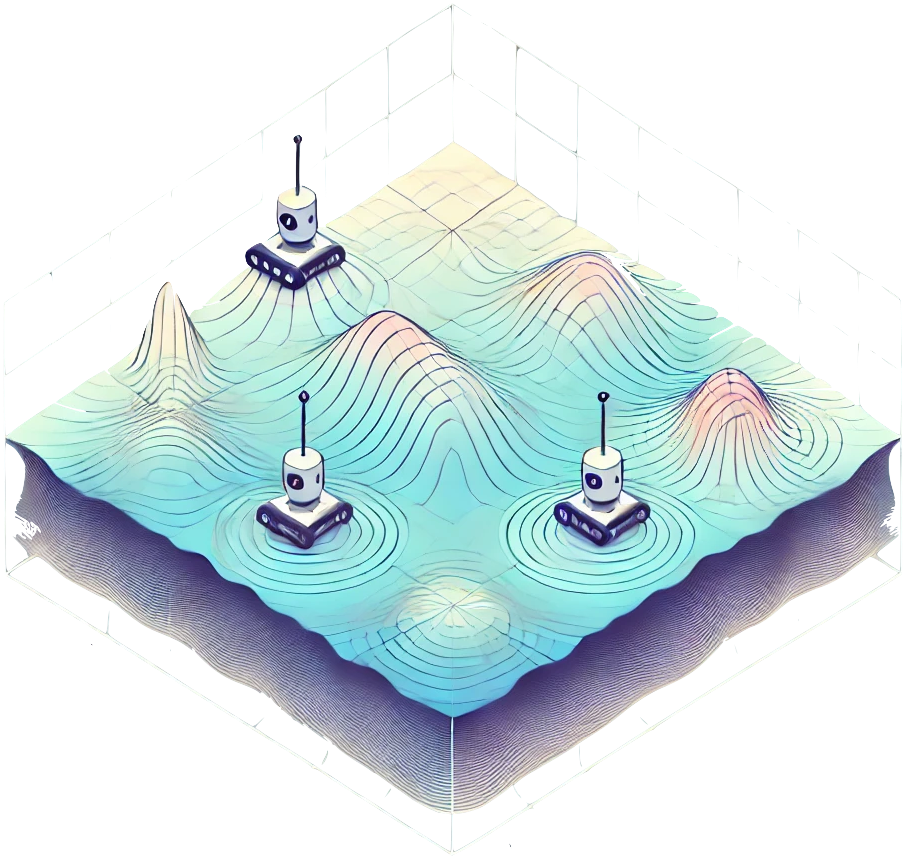
\includegraphics[width = 0.4\linewidth,valign=c]{illustration figure_1}} 
	\subfloat[Continuous world trajectory \label{fig:SecurityBreak}]{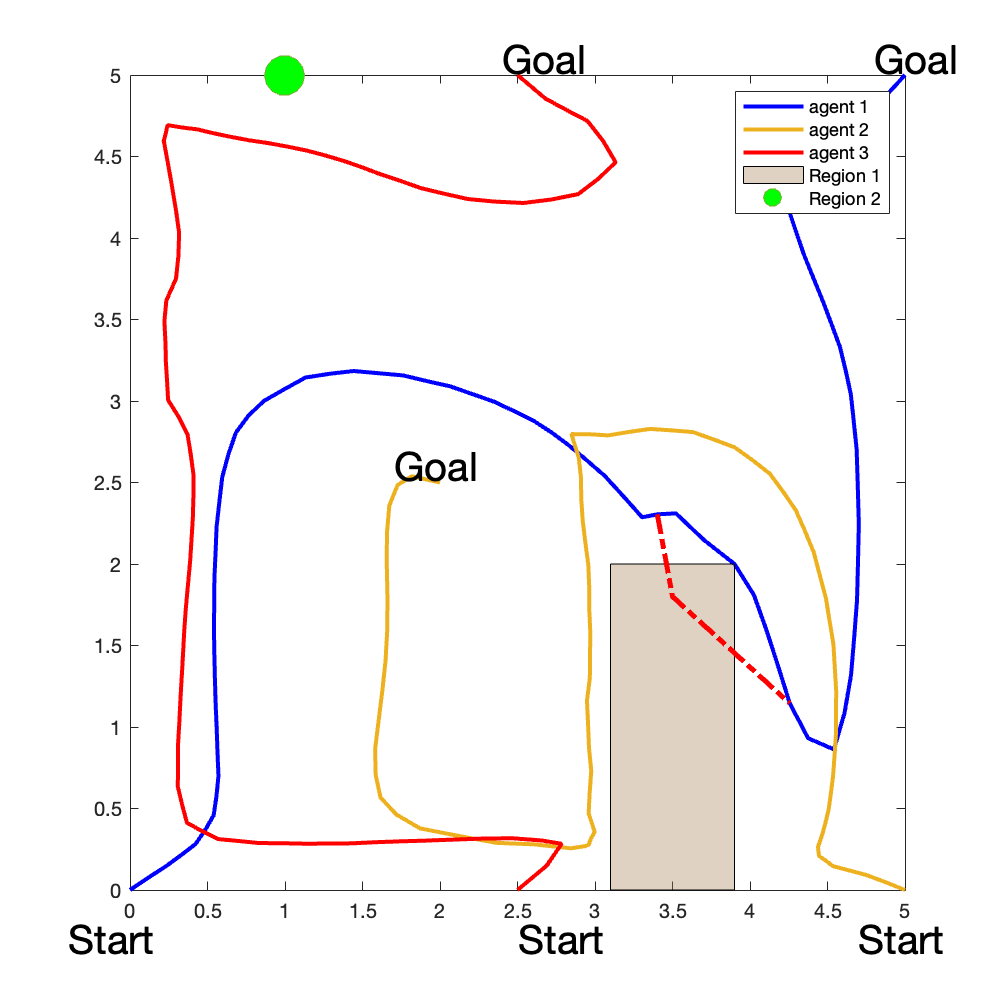
\includegraphics[width=0.4\linewidth,valign=c]{SecurityBreak_v2}}
	% \subfloat[\new{Grid world result.}\label{fig:Grid-example-application}]{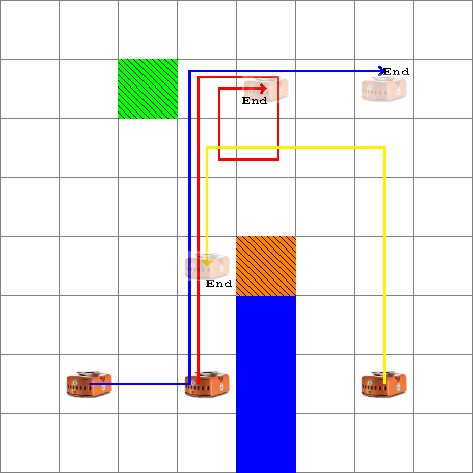
\includegraphics[width = 0.4	\linewidth]{Grid_world}}
	\caption{\new{(2a) Illustration of a 3 robot map exploration task case. (2b) The unsecured trajectory design optimized for a map exploration task. Potential security breaches, indicated by red dashed lines, highlight paths that could allow unauthorized access to forbidden regions.}}
\end{figure}
{\news In the absence of further security requirements, the robots are expected to spread out and follow a boustrophedon pattern, efficiently exploring as much of the task space as possible (as illustrated in Fig.2b). This exploration strategy optimizes coverage and minimizes reconstruction uncertainty across the field. }


%%%%%%%%%%%%% Comment 1.2
\begin{cmt}{}{}
	Personally, I think to much space is dedicated to the details of how
	reachability constraints are implemented in the ADMM formulation (Sec.
	D, E, F, G, H). Although they are important details, I think this part
	can be condensed more, and some of the details can be deferred to the
	Appendix, so that some space can be dedicated more to improve the
	clarity of the other sections.
	\tcblower
	\underline{\textbf{Response:}} As suggested, we have condensed this section and moved the “Transformation to Canonical Frame” part into the appendix to streamline the main text and improve readability. We believe that the remaining details on the implementation of the reachability constraints are essential and provide critical context for understanding the proposed method. We appreciate your suggestion, which has helped us enhance the balance and clarity of the manuscript. 
\end{cmt}
\rv
\renewcommand\thesubsection{D}
 \subsection{Transformation to canonical coordinates}\label{sec:rotation2Standard}
{\news	\newcommand{\oFE}{o}
 To use the definition of reachability ellipsoid from the section above as computational constraints for ADMM, we first apply a differentiable rigid body transformation to reposition the ellipse $\cE$ from the global frame $\cF$ to a canonical frame $\cF_\cE$, where the origin of $\cF_\cE$ is at the ellipsoid's center $\oFE = \frac{1}{2}(q_1+q_2)$, and the first axis of $\cF_\cE$ is aligned with the foci (see Fig.3a for an illustration). 
From this definition, a unit vector along the first axis of the ellipsoid in the frames $\cF$ and $\cF_\cE$ is given by $\nu_\cF = \frac{q_2-q_1}{\norm{q_2-q_1}}$ and $\nu_\cE =[1,0,0]^T$, respectively.
The full transformation from coordinates $q^\cE\in\cF$ to $q\in\cF$, and its inverse, are then parametrized by a rotation $R^\cF_\cE$ and a translation $o^\cF_\cE$ as (we drop the subscript and superscript from $R^\cF_\cE$ and $o^\cF_\cE$ to simplify the notation):
\setcounter{equation}{9}
\begin{equation}\label{eq:transformations}
  q=R\Eframe{q}+\oFE,\quad
  \Eframe{q}=R\transpose(q-\oFE).
\end{equation}
where the rotation matrix $R=H(\nu_\cF(q_1,q_2),\nu_\cE)$ is a \emph{Householder rotation} $H$ (a differentiable linear transformation describing the minimal rotation between the two vectors, see Appendix B for details).  To simplify the notation, in the following, we will consider $H$ to be a function of $q_1,q_2$ directly, i.e. $H(q_1,q_2)$. More details on (10) are given in Appendix A.
  Reachability constraints are formulated with respect to different types of forbidden regions a point, a plane, a segment, and a convex polygon.}
\renewcommand\thesubsection{F}
\subsection{Plane-ellipsoid reachability constraint}\label{sec:ellipsoide-plane}
\new{For a hyperplane shaped forbidden region $\mathcal{L}(q) = \{q\in\mathbb{R}^m: \vn\transpose q = d\}$ (Fig.3c), the reachability constraint is $\mathcal{L} \cap \mathcal{E}(q_1,q_2,a) = \emptyset$. When transformed into the canonical frame, the hyperplane can be written as $\Eframe \cL(\Eframe{q}) = \{  \Eframe{q}\in\mathbb{R}^m:  \vn_\cE\transpose \Eframe{q} = d_{\cE}\}$, with $\vn_\cE = H(q_1,q_2)\vn, \quad d_\cE =-\vn\transpose o + d$.}
%%
\renewcommand\thesubsection{G}
\def\sZ{\mathcal{Z}}
\subsection{Convex-polygon-ellipse reachability constraint}\label{sec:ellipse-region-constraint}
{\news  
The reachability constraints for a convex polygon is treated as a union of reachability constraints for aeach indivisual segments that define the hyperplane. We define
\setcounter{constraint}{3}
\setcounter{equation}{29}
\begin{constraint}[Convex-polygon-ellipsoid reachability constraint]\label{constraint:polygon-ellipsoid}
\begin{align}
D(\vq) &= \bmat{D_{seg1}(\vq)\\D_{seg2}(\vq)\\ \vdots} \label{eq:region_ellipsoid_constraint}\\
  \sZ &= \{\vq\in\mathbb{R}^{nm}:\norm{D(\vq)} = 0 \},\\
   \Pi_\sZ(\vz) & = 0, 
\end{align}
\end{constraint}
where $D_{seg}$ are the constraint functions for all line segments used to define the convex polygon region. 
For hyperplane $\Eframe \cL(\Eframe q) = \{ \Eframe q\in\mathbb{R}^m:  \vn_\cE\transpose \Eframe q = d_{\cE}\}$ with endpoints $\Eframe {p_1}$ and $\Eframe{p_2}$; this segment is defined as:
\begin{equation}
\bmat{(\Eframe {p_1}- \Eframe{p_2})\transpose\\( \Eframe{p_2} - \Eframe{p_1})\transpose}  \Eframe p \leq \bmat{ \Eframe{p_2}\transpose\\- \Eframe{p_1}\transpose}( \Eframe{p_1}- \Eframe{p_2}), \quad \vn_\cE\transpose \Eframe q = d_{\cE}.
\end{equation}
When the \emph{tangent interpolation point} $\Eframe{p_{\cL}}$ stays within the segment (i.e. red region in Fig. 3d), the constraint is a plane-ellipse constraint in Section II-F. Otherwise (i.e. brown region in Fig. 3d), the constraint is a point-ellipse constraint in Section II-F.

\begin{constraint}[Line-segment-ellipsoid reachability constraint]
\begin{align}
D_{seg}(\vq) &=  \begin{cases}
D_{p_{1}}(\vq) & (\Eframe{p_1}-\Eframe{p_2})\transpose (\Eframe{p_{\cL}}-\Eframe{p_2})<0\\
D_{p_{2}}(\vq) & (\Eframe{p_2}-\Eframe{p_1})\transpose (\Eframe{p_{\cL}} -\Eframe{p_1})<0\\
D_\Eframe{p_{\cL}}(\vq) & \textrm{otherwise}
\end{cases} \label{eq:segment_ellipsoid_constraint}\\
  \sZ &= \{\vq\in\mathbb{R}^{nm}:\norm{D_{seg}(\vq)} = 0 \},\\
   \Pi_\sZ(\vz) & = 0, 
\end{align}
\end{constraint}
where $D_{p_{1}}$ and $D_{p_{2}}$ are the point-ellipsoid constraint projection function (11) respect to $\Eframe{p_{1}}$ and $\Eframe{p_{2}}$, and $D_\Eframe{p_{\cL}}$ is the plane-ellipsoid constraint (22). with respect to frame $\Eframe {\cL}$.
This constraint needs to be supplemented with a convex obstacle constraint for the polygon (i.e. keep foci waypoints outside the region, introduced in [6]) to prevent cases where the ellipse is a subset of the region.
}

\vspace{0.2cm}
%%%%%%%%%%%%% Comment 1.3
\begin{cmt}{}{}
	The word “checkpoint” appears abruptly in page 6 without concrete
	definition, although it seems like it is an important component of the
	formulation, and an important design choice for the results. For
	example, in the way Figure 3 is presented, I don't get a good idea why
	the checkpoint location is there in (c). 
	\re 
	\noindent
 For the feedback reguarding the term "checkpoint", the original intent of “checkpoint” in Section 2 was to illustrate the limitations of the method proposed, specifically to show that even if APMAPF yields a valid solution, transforming this solution to a continuous domain may still need additional security measure to guarantee security. To address the concern, we have replaced the term “checkpoints” with “key locations” in Section 2 to avoid confusion. Additionally, we have added a formal definition of “checkpoints” and the “checkpoint graph” later in Section 3 to provide a clear and precise explanation of these concepts. These updates ensure that the term is used consistently and that its role in the methodology is explicitly defined. 
\end{cmt}
\rv
\renewcommand\thesubsection{H}
\subsection{Secured planning results and limitation}\label{sec:ADMM-simulation}
We employ the \new{attack-proof MAPF(APMAPF)} solver [2] on an 8 by 8 grid world with a similar setup to generate a MAPF plan with a co-observation schedule in a grid-world application (Fig.4a). This result is transformed to a continuous configuration space and serves as the initial trajectory input for the ADMM solver with an additional task function targeting the map exploration task. Co-observation schedules are set up using the APMAPF algorithm for two forbidden regions. Reachability constraints are added to ensure an empty intersection between all robots' reachability regions during co-observations and the forbidden regions. {\news It is important to emphasize that an APMAPF solution does not guarantee existence, nor does it ensure a successful transition to the continuous configuration space. In this case, while an APMAPF solution may be found, the secured, attack-proof solution becomes infeasible in the continuous setting because the robots' mobility is no longer restricted to adjacent grids. Additional security measures, such as stationary security cameras or surveillance robots, need to be incorporated. For instance, in this scenario, we deploy a security camera as additional security measure to observe agent 3 at time $8$ to ensure security.}

The simulation result, shown in Fig.4b, displays reachability regions as black ellipsoids, demonstrating empty intersections with Zones 2 and 3. Explicit constraints between reachability regions and obstacles are not activated, assuming basic obstacle avoidance capabilities in robots. The intersections between obstacles and ellipsoids, as observed between agent 3 and Zone 1, are deemed tolerable. All constraints are satisfied, and agents have effectively spread across the map for optimal exploration tasks.

1) Limitations:
Our solution demonstrates the potential of planning with reachability and co-observation to enhance the security of multi-agent systems. {\news However, two primary challenges need to be addressed. Firstly, achieving a co-observation and reachability-secured plan is not always feasible, particularly when obstacles or restricted regions separate the robots, preventing them from establishing co-observation schedules or finding reachability-secured paths. For example, agent 3 in~Fig.4b requires additional security measures to create secured reachability areas. Secondly, security requirements can impact overall system performance, as illustrated by the comparison between~Fig.2b and Fig.4b. The introduction of security constraints resulted in the top left corner remaining unexplored by any robots. This trade-off between security and system performance is particularly significant as system performance is a key factor in the decision of multi-agent system deployments. These challenges are further addressed in Section III, ensuring the effective integration of reachability and co-observation in securing multi-agent systems.}

\vspace{0.3cm}

\begin{cmt}{}{}
	Similarly, how the
	trajectories are broken down to multiple ellipsoid components are not
	clear, is it a design choice to make the constraints less conservative
	than setting a single ellipsoid with the start and goal point?
	\re 
	The reachability ellipsoids are designed to work in conjunction with the co-observation technique. Instead of using a single ellipsoid defined by the start and goal points, the trajectory is divided into smaller ellipsoids based on co-observation times. This approach ensures that the constraints are aligned with the co-observation schedule, reducing conservativeness while maintaining security guarantees. We also make modification to Definition 4 (Remark 1 in the original manuscript) to make this more clear.
\end{cmt}
\rv
{\news \setcounter{definition}{3}
 \begin{definition}\label{rmk:revised-security}
	A multi-robot trajectory is secured against plan-deviation attacks if there exists a co-observation plan such that the reachability region between each consecutive co-observation does not intersect with any forbidden regions.
\end{definition}}

\vspace{0.3cm}
\begin{cmt}{}{}
	Similarly, in page 7, “key locations” and “checkpoint graph” are
	mentioned without clear explanations what they are.
	\re  
	In Section III, we add additional definition to 'checkpoint' and 'checkpoint graph'
\end{cmt}
\rv

{\news
Our strategy is based on the following concept:
\setcounter{definition}{5}
\setcounter{remark}{1}
\begin{definition}
The $i$-th \emph{checkpoint} $v_{pi}=(q_{p},t_{i})$ for sub-team $p$ is defined as a location $q_{pi}=q_{p}(t_i)$ and time $t_{i}$. It represents either the first or last instance where a robot is co-observed by a teammate, and serves as a point where the robot can leave or join a new team.
% at which a robot is co-observed by its teammates, and where it can leave or join a new team. 
\end{definition}
For simplicity, let $\cI_{v_{i}}$ denote the sub-team to which $v_{i}$ belongs. %, and $q_{v_{pi}} =q_{pi}$ and $t_{v_{pi}}$ be the corresponding location and time for checkpoint $v_{pi}$.
To ensure the security of the reference trajectory, the reachability region between consecutive checkpoints must avoid intersections with forbidden regions. This requirement can be formally stated as:
\begin{remark}\label{rmk:checkpoints}
  A set of checkpoints $V_{p}=\{ v_{p0}, \dots ,v_{pT}\}$ (arranged in ascending order of $t_{v_{pi}}$) can secure the reference trajectory for sub-team $p$, if $\mathcal{E}(q_{v_{pi}}, q_{v_{p(i+1)}}, t_{v_{pi}},t_{v_{p(i+1)}}) \intersect F = \emptyset$ for every $i$, where $F$ is the union of all forbidden regions.
  \end{remark}
}
{\news 
\begin{definition}
  The planned trajectory $\{q_p\}_{p=1}^{N_p}$ is represented as a directed \emph{checkpoint graph} $G=(V, E)$, where $V = (\union_p V_p) \union V_c$ is the set of verticies representing waypoints on the planned trajectory and $E = E_{t} \union E_{c}$ is the set of edges representing feasible paths connecting $V$. The components of the checkpoint graph are defined as follows:
  \begin{description}
    \item[Checkpoints $V_p$] where additional robots are required for security through co-observation.
    \item[Trajectory edges $E_t$] represent the original planned path of the primary robot.
    \item[Connection vertices $V_c$] represent non-checkpoint locations linked via $E_c$.
    \item[Cross-trajectory edges $E_c$] represent feasible paths where robots deviate from the original trajectory to join other teams or provide co-observation support, at least one endpoint be a checkpoint. 
  \end{description}
\end{definition}}
\vspace{0.3cm}
\begin{cmt}{}{}
	The plots are not reader-friendly at all. In all figures, trajectory
	lines are too thin. The legend text is too small. In figure 2, there is
	no number scale for (b) and I am even not sure if this corresponds to
	the same scenario as (a) and (c). In Figure 5, the color of the
	sub-team robots seem like not matching with the main robots.
	\re We have re-plotted the figures to make them more reader-friendly by thickening trajectory lines, enlarging legend text, and ensuring consistent coloring between sub-team robots and main robots in Figure 7 and Figure 8  (Figure 5 and 6 in original manuscript).

	For Figure 2, we appreciate the comment regarding the lack of a number scale especially on (b,c,d). The intention of these figures are to illustrate the geometric relationships between ellipsoids and different shapes, as well as the transformation of coordinates. To maintain focus on these aspects, we chose to omit the number scale and believe that it is not essential for conveying the intended concept.
\end{cmt}
\rv
\setcounter{figure}{1}
\begin{figure}[H]
	\centering
	\subfloat[\new{Map exploration task.}\label{fig:illustration}]{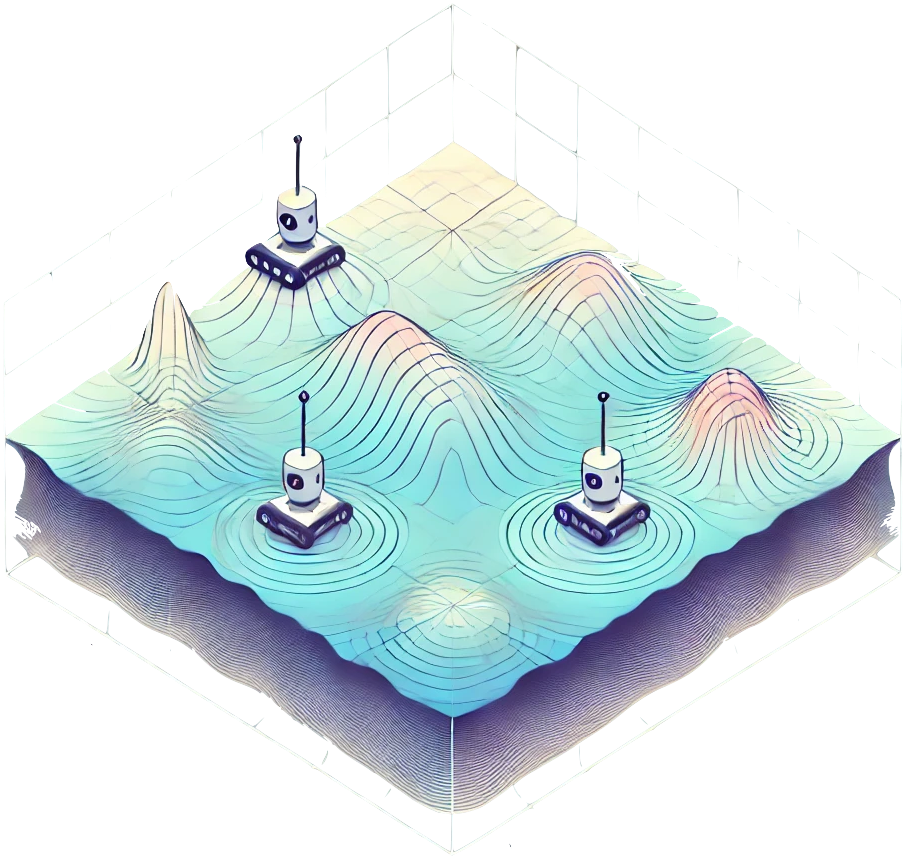
\includegraphics[width = 0.4	\linewidth,valign=c]{illustration figure_1}} 
	\subfloat[Continuous world trajectory \label{fig:SecurityBreak}]{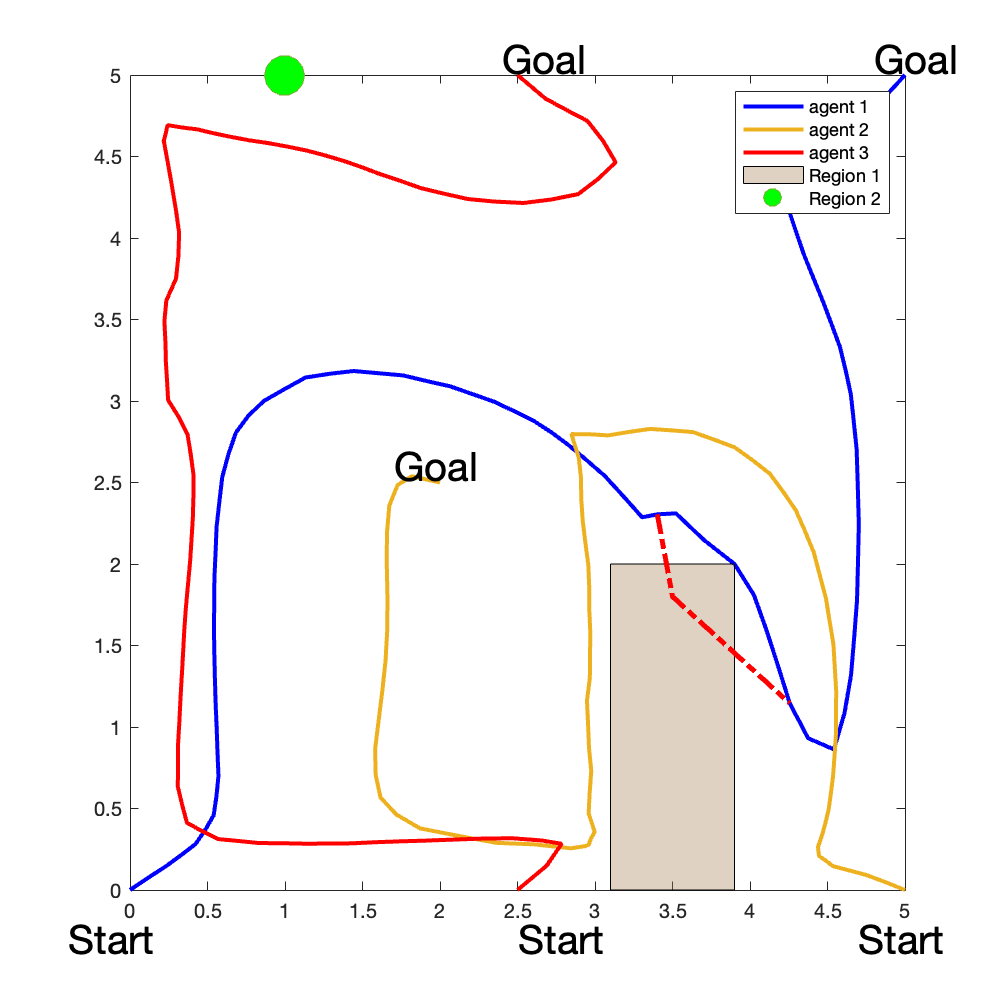
\includegraphics[width=0.4	\linewidth,valign=c]{SecurityBreak_v2}}
	% \subfloat[\new{Grid world result.}\label{fig:Grid-example-application}]{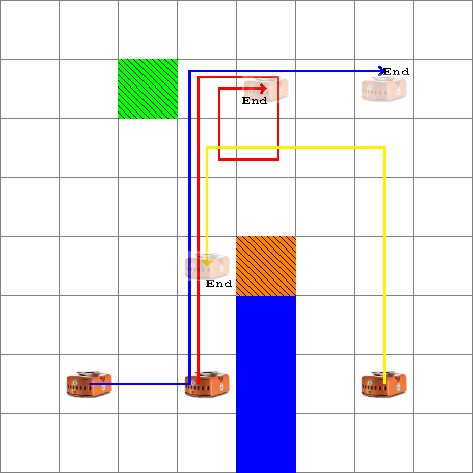
\includegraphics[width = 0.4	\linewidth]{Grid_world}}
	\caption{\new{(2a) Illustration of a 3 robot map exploration task case. (2b) The unsecured trajectory design optimized for a map exploration task. Potential security breaches, indicated by red dashed lines, highlight paths that could allow unauthorized access to forbidden regions.}}
  \end{figure}
\setcounter{figure}{3}
  \begin{figure}[H]
	\centering
	% \subfloat[Grid-world trajectory. \label{fig:Grid-example-application}]{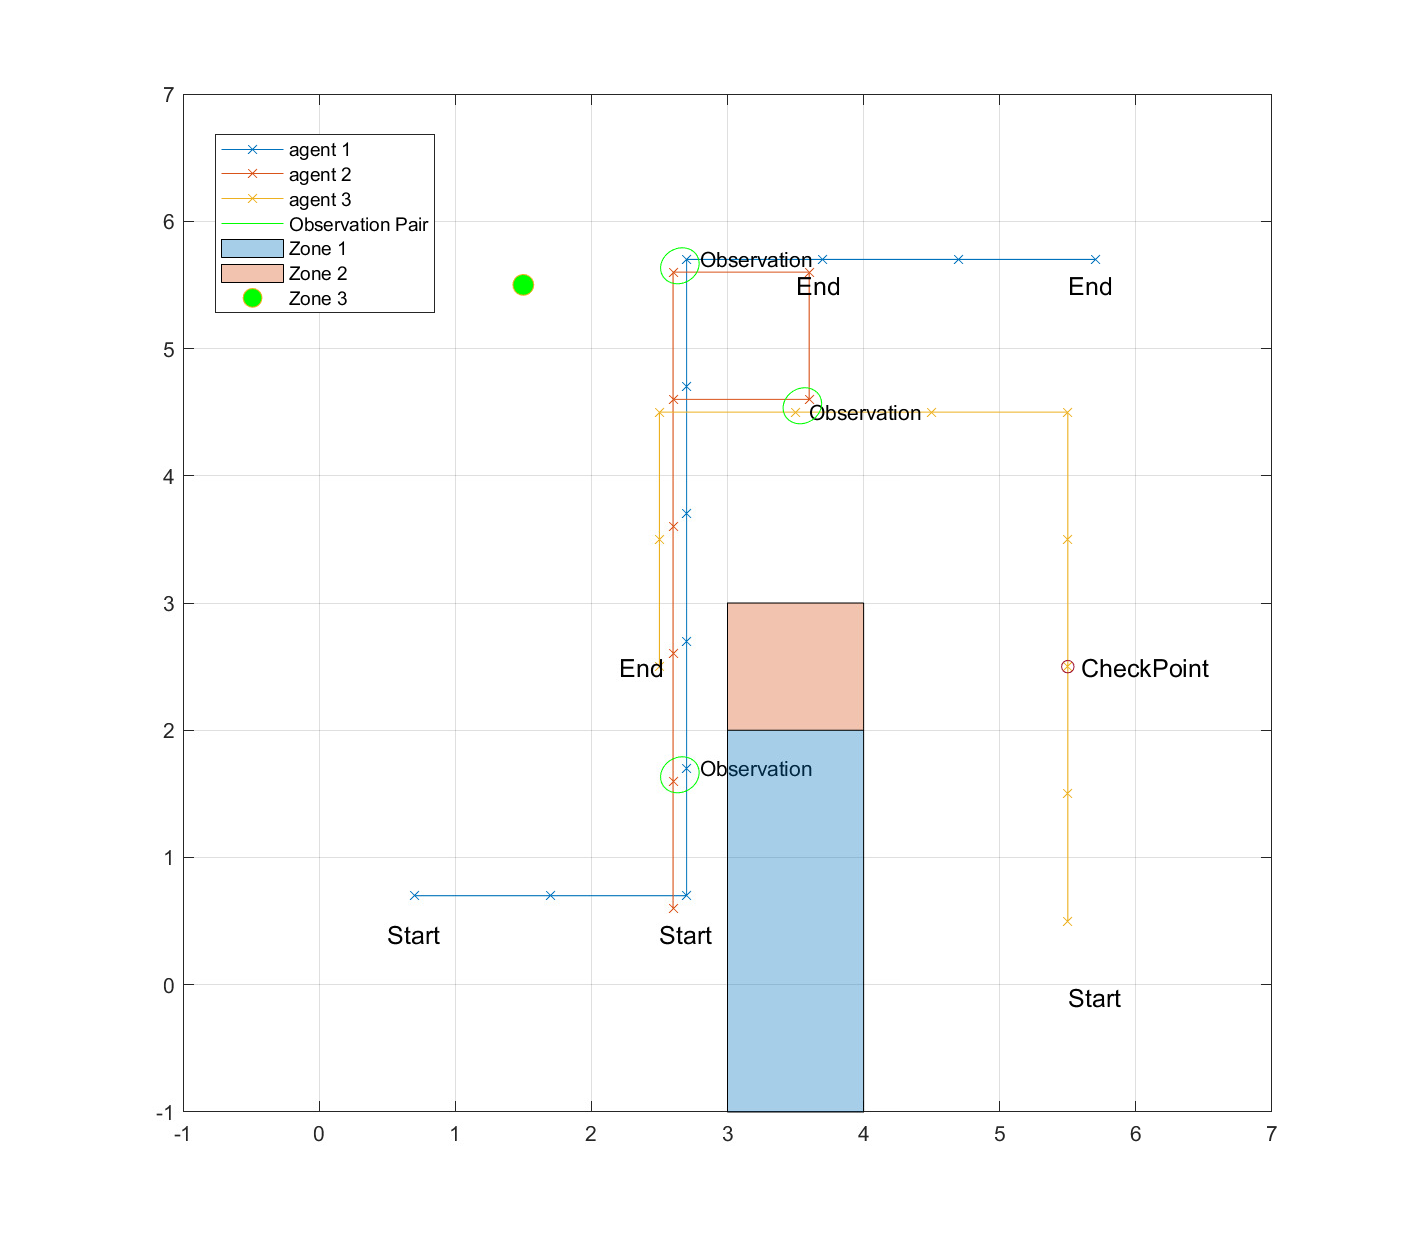
\includegraphics[width=0.4	\linewidth, trim = 2cm 0.5cm 0cm 2cm]{Kacper_result}}
	\subfloat[\new{Grid world result.}\label{fig:Grid-example-application}]{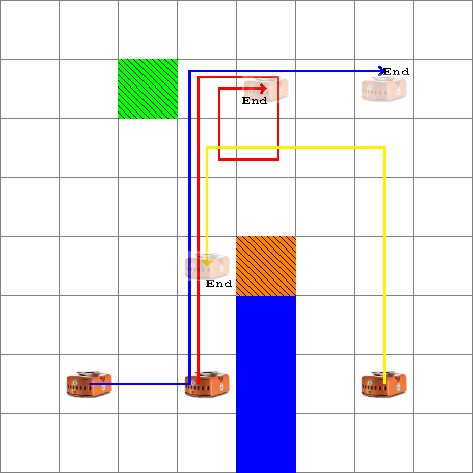
\includegraphics[width = 0.4	\linewidth,valign=c]{Grid_world}}
	% \subfloat[Continuous world trajectory \label{fig:SecurityBreak}]{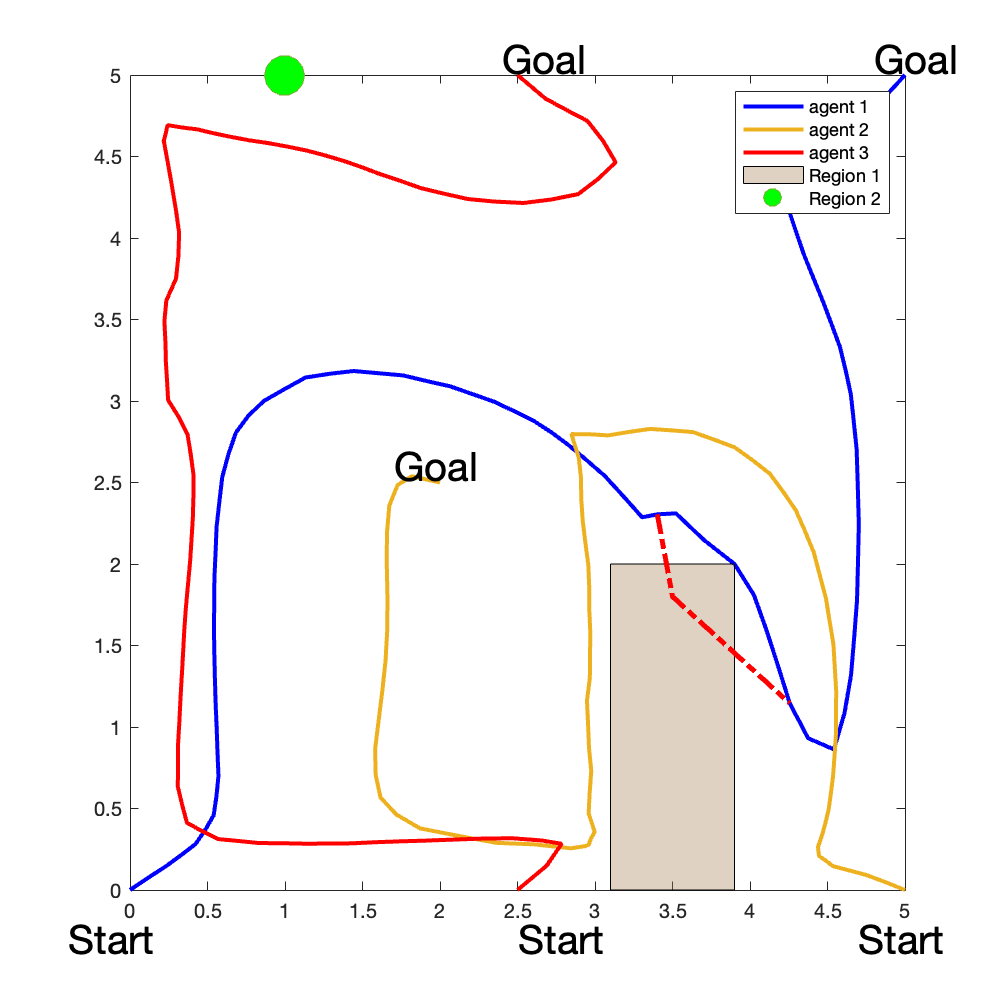
\includegraphics[width=0.4	\linewidth,valign=c]{SecurityBreak_v2}}
	\subfloat[Securd result \label{fig:ReachabilitySimulation}]{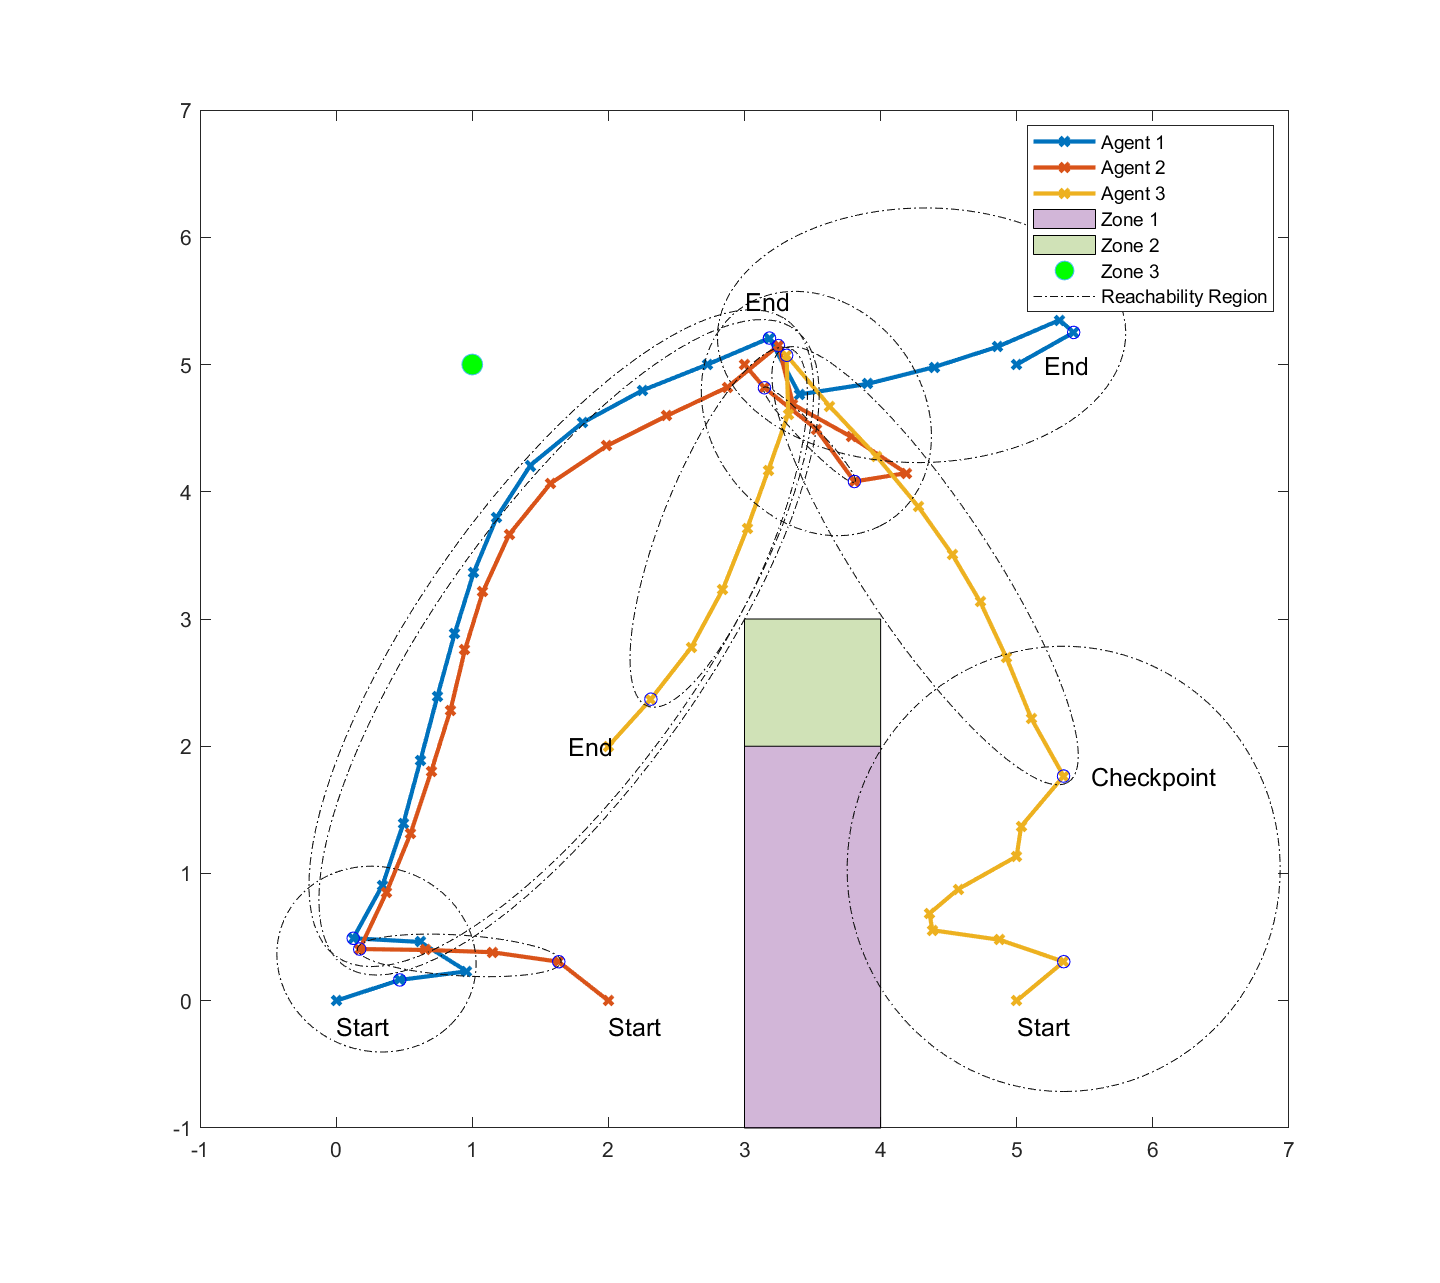
\includegraphics[width=0.52\linewidth,trim =2cm 1.5cm 2cm 1cm, clip,valign=c]{FinalResult}}
	\caption{{\news Trajectory design a three-robot system based on the grid world result. Zone 1 is an obstacle, Zone 2 and Zone 3 are forbidden regions. (\ref{fig:Grid-example-application}) Result of the APMAPF algorithm in 8$\times$8 grid-world without map exploring objective. (\ref{fig:ReachabilitySimulation}) The secured trajectory with the incorporation of co-observation generated by APMAPF and additional reachability constraints.}}
	\label{fig:example-application}
  \end{figure}
  \setcounter{figure}{6}
  \begin{figure}[H]
	\centering
	\subfloat[Cross-trajectory co-observation plan \label{fig:previous_result_plan}]{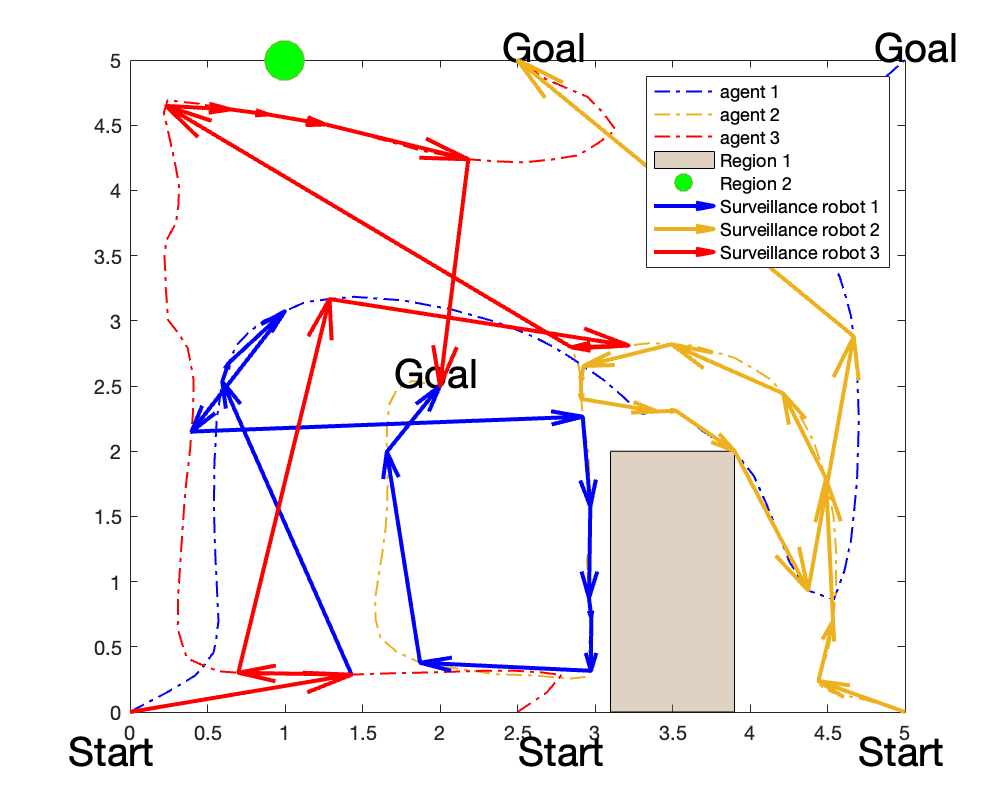
\includegraphics[width=0.4\linewidth, trim = 2cm 1cm 1cm 1cm,clip,valign=b]{old_result_v2}}
	\subfloat[Checkpoint graph and result flows \label{fig:previous_result_graph}]{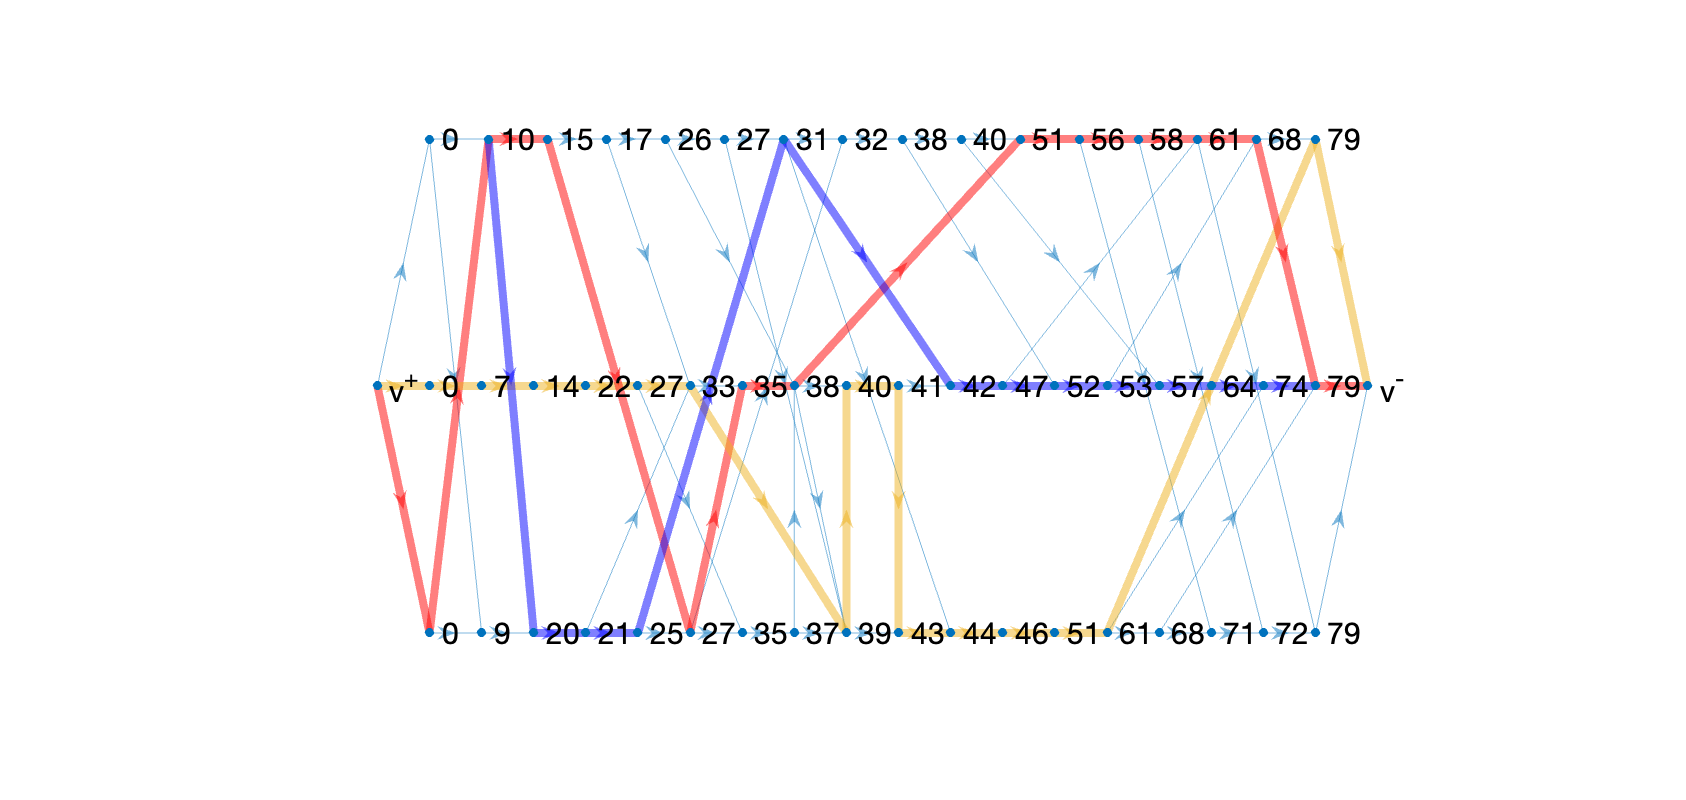
\includegraphics[width=0.4\linewidth, trim = 10cm 3cm 7cm 3cm,clip,valign=b]{old_result_graph_v2}}
	\caption{\new{(\ref{fig:previous_result_plan}) The cross-trajectory co-observation plan is shown as arrows on top of the original plan in \cref{fig:previous_result_plan}. (\ref{fig:previous_result_graph}) The checkpoint graph and resulting flows highlighted.}}
	\label{fig:3-team-ctco}
  \end{figure}

  \begin{figure}[H]
	\centering
	%\subfloat[Unsecured plan\label{fig:unsecured-plan}]{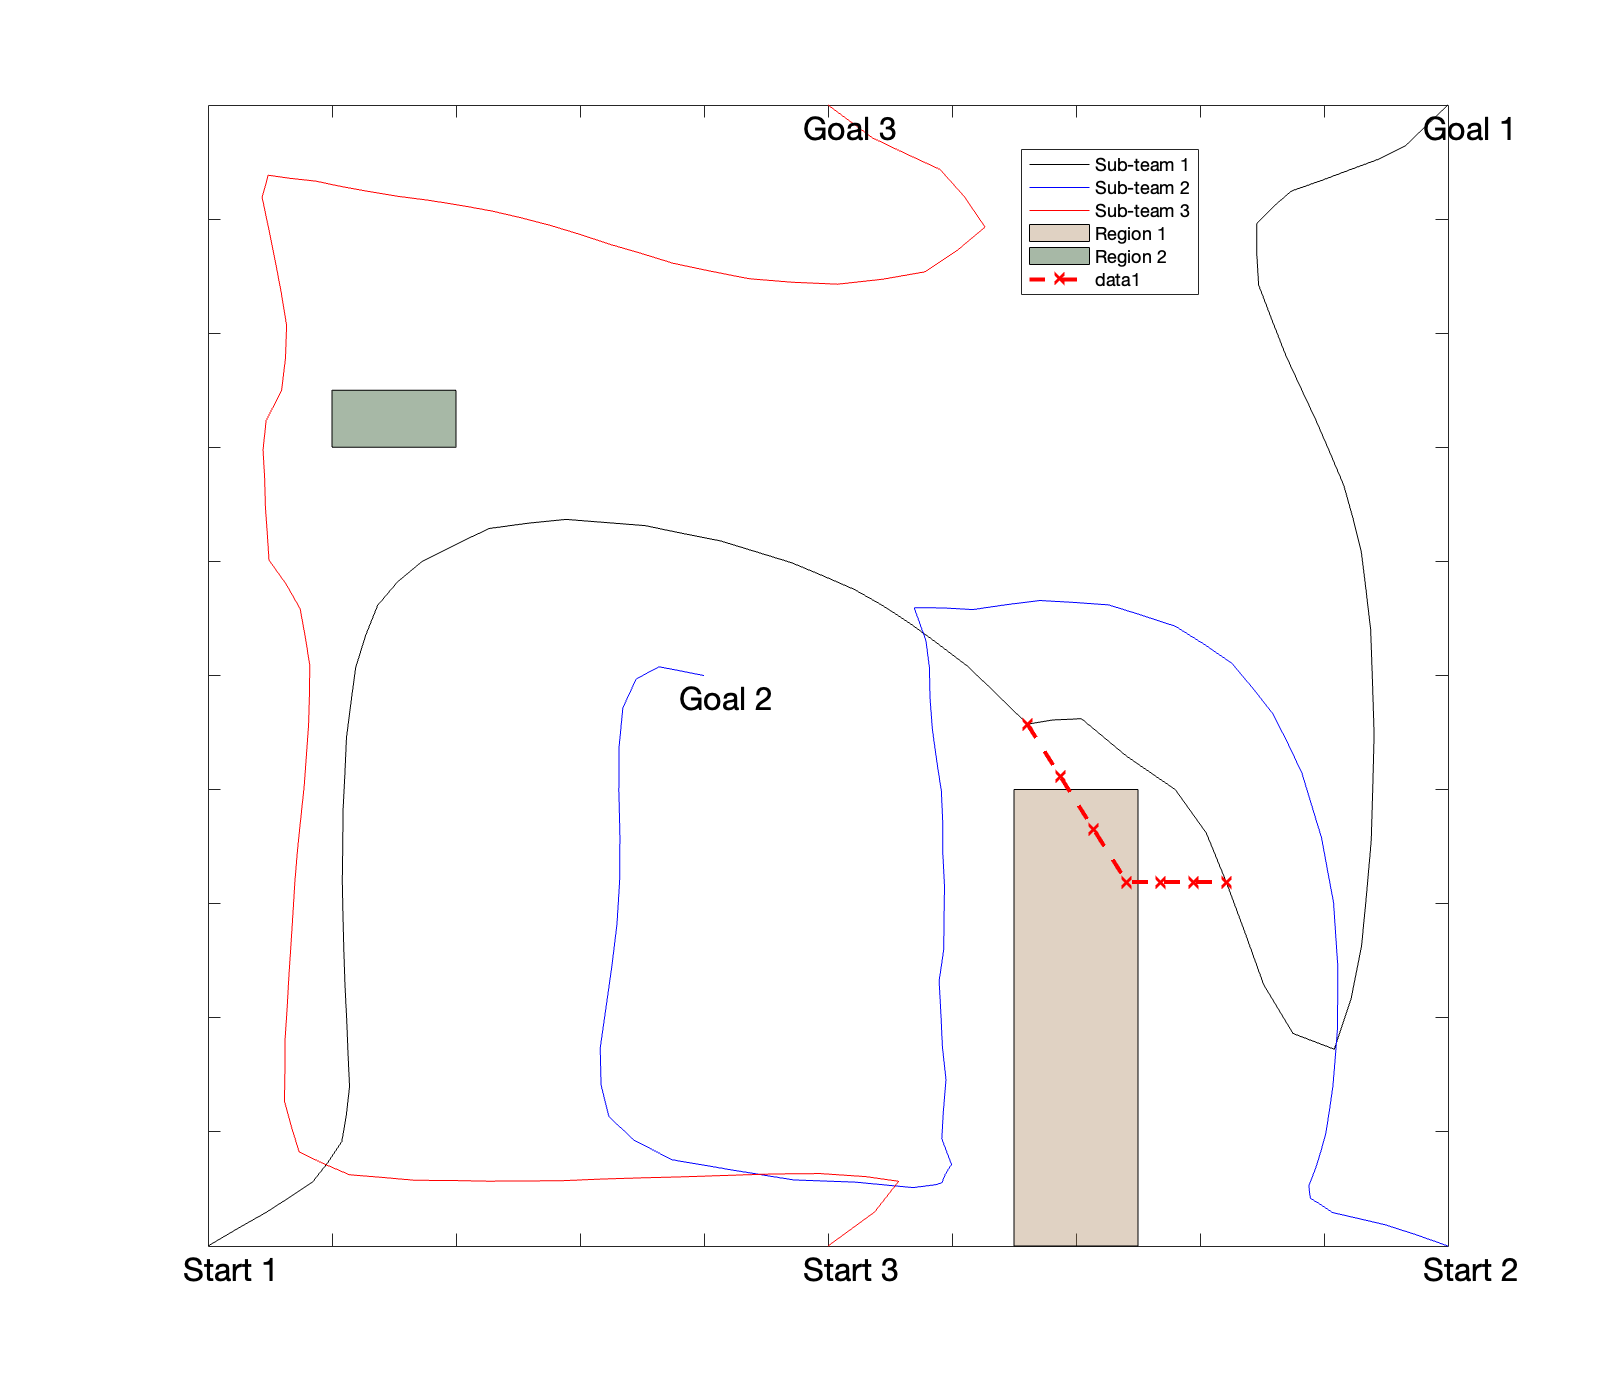
\includegraphics[width=0.31\linewidth, trim = 3cm 2cm 3cm 2cm, clip,valign=c]{SecurityBreak}}
	\subfloat[4-agent case\label{fig:Result-plan}]{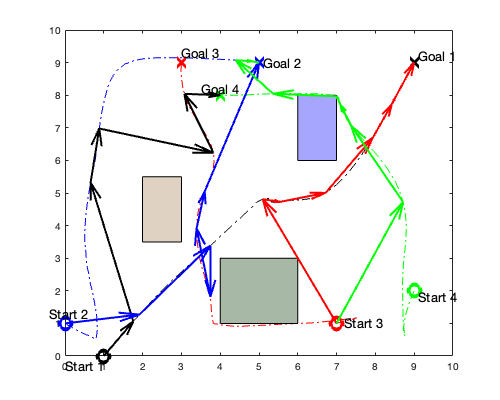
\includegraphics[width=0.4\linewidth,trim = 1cm 1cm 1.5cm 0cm, clip,valign=c]{Traj_result_v3.png}}
	%\subfloat[Graph flow result\label{fig:result-graph}]{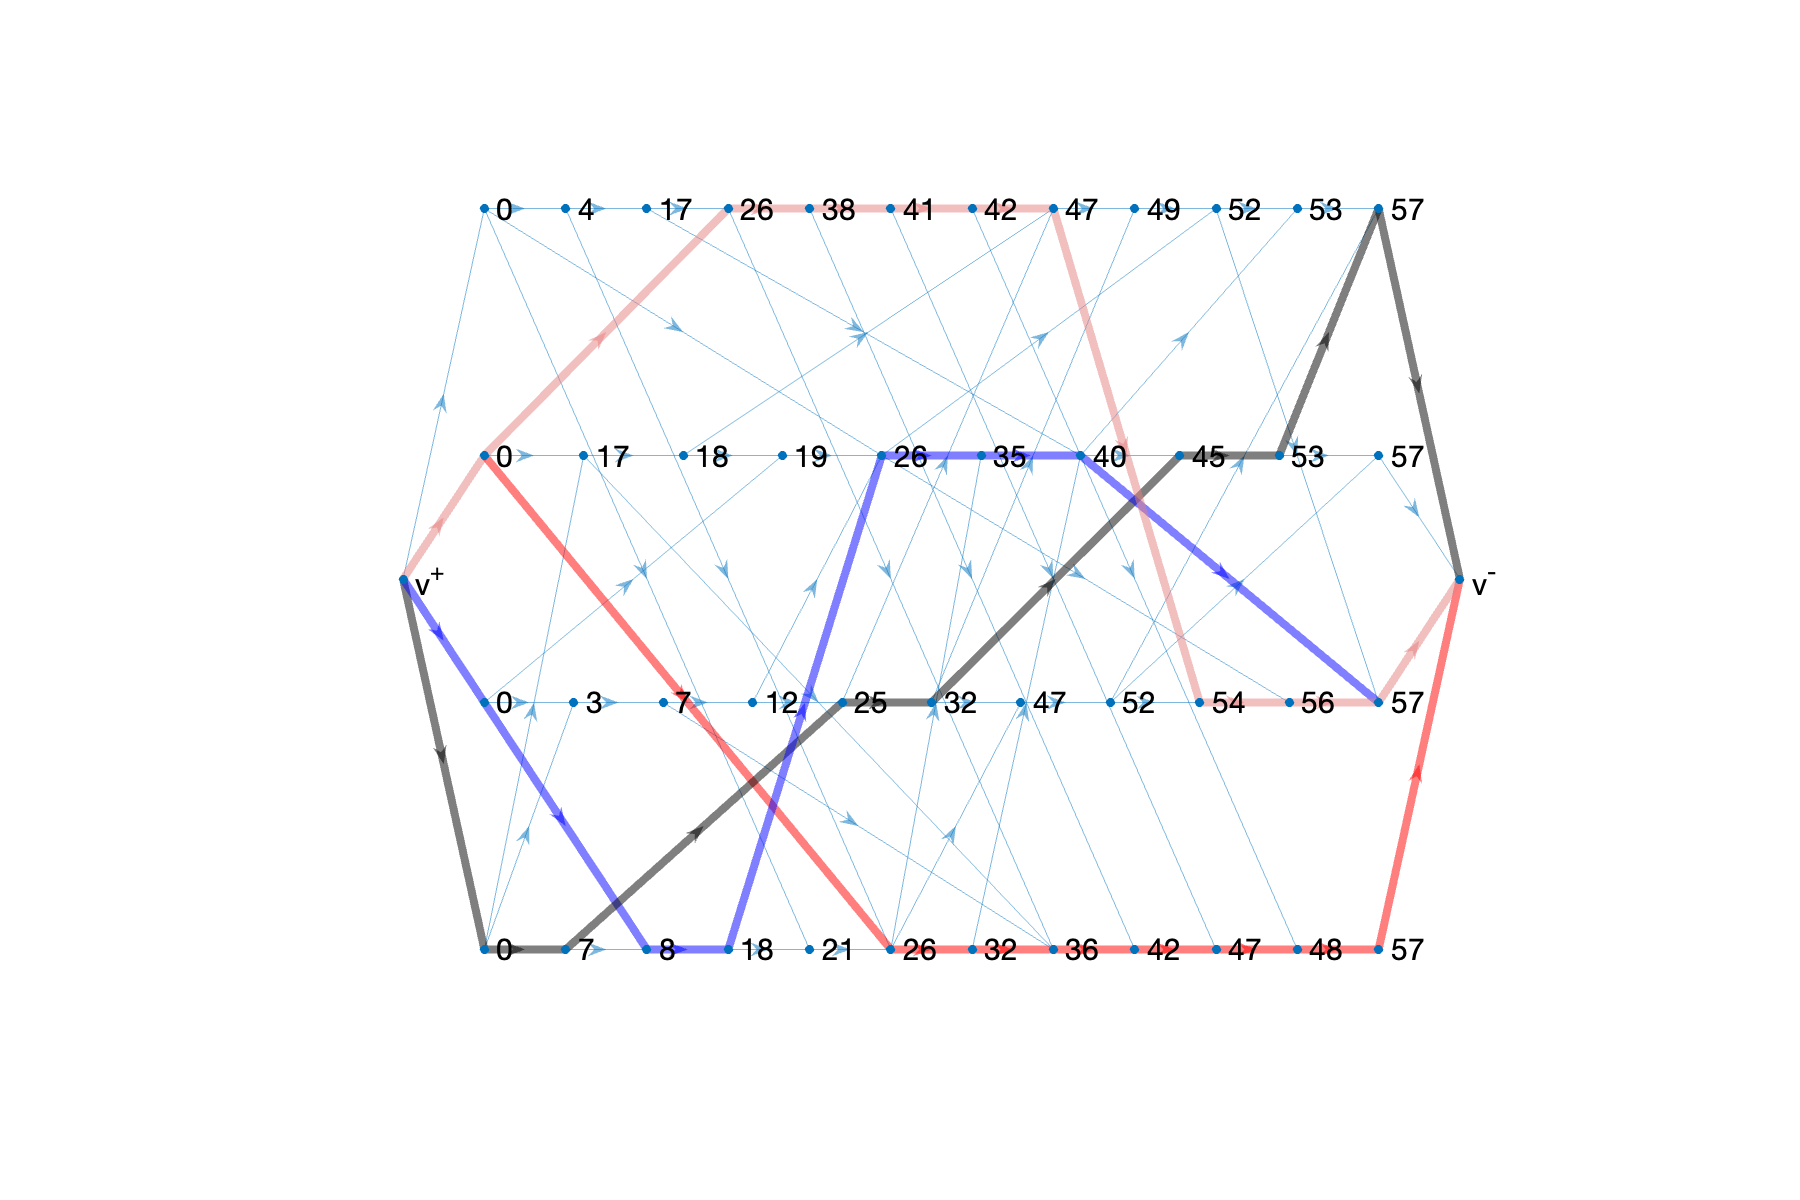
\includegraphics[width=0.47\linewidth,trim = 4cm 0cm 4cm 0cm, clip,valign=c]{Graph_result}}
	\subfloat[7-agent case\label{fig:Result-plan-7-team}]{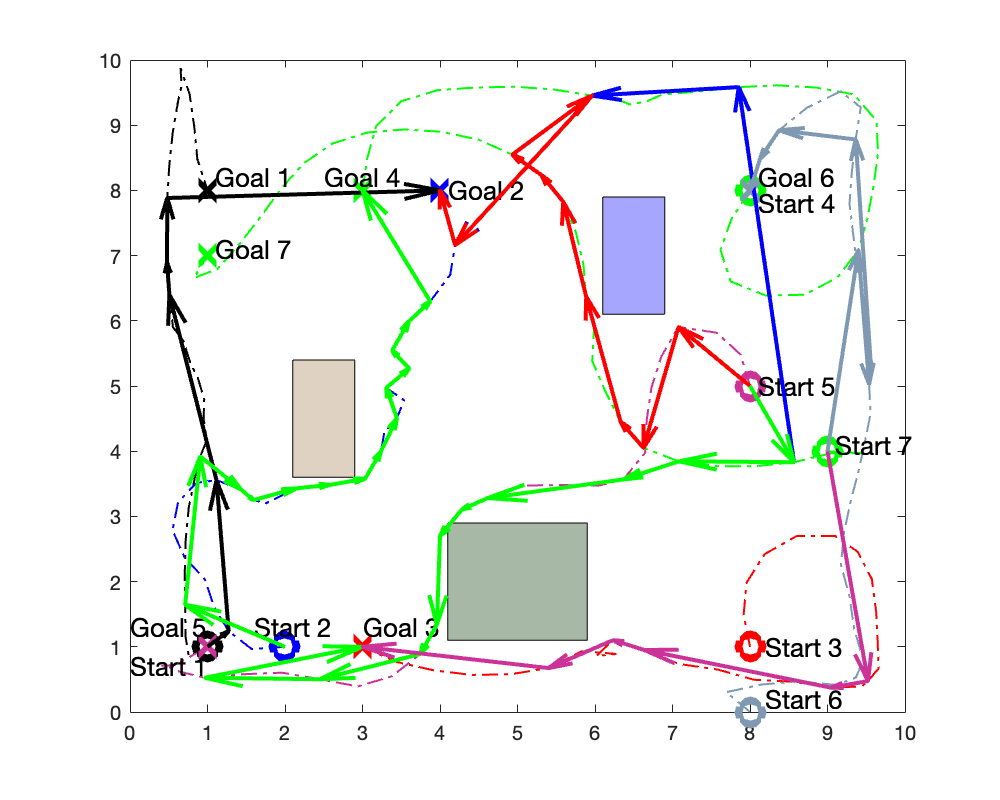
\includegraphics[width=0.4\linewidth,trim = 3.5cm 2cm 1.5cm 0cm, clip,valign=c]{7-team-plan_v2.png}}
	%\subfloat[Graph flow result\label{fig:result-graph-7-team}]{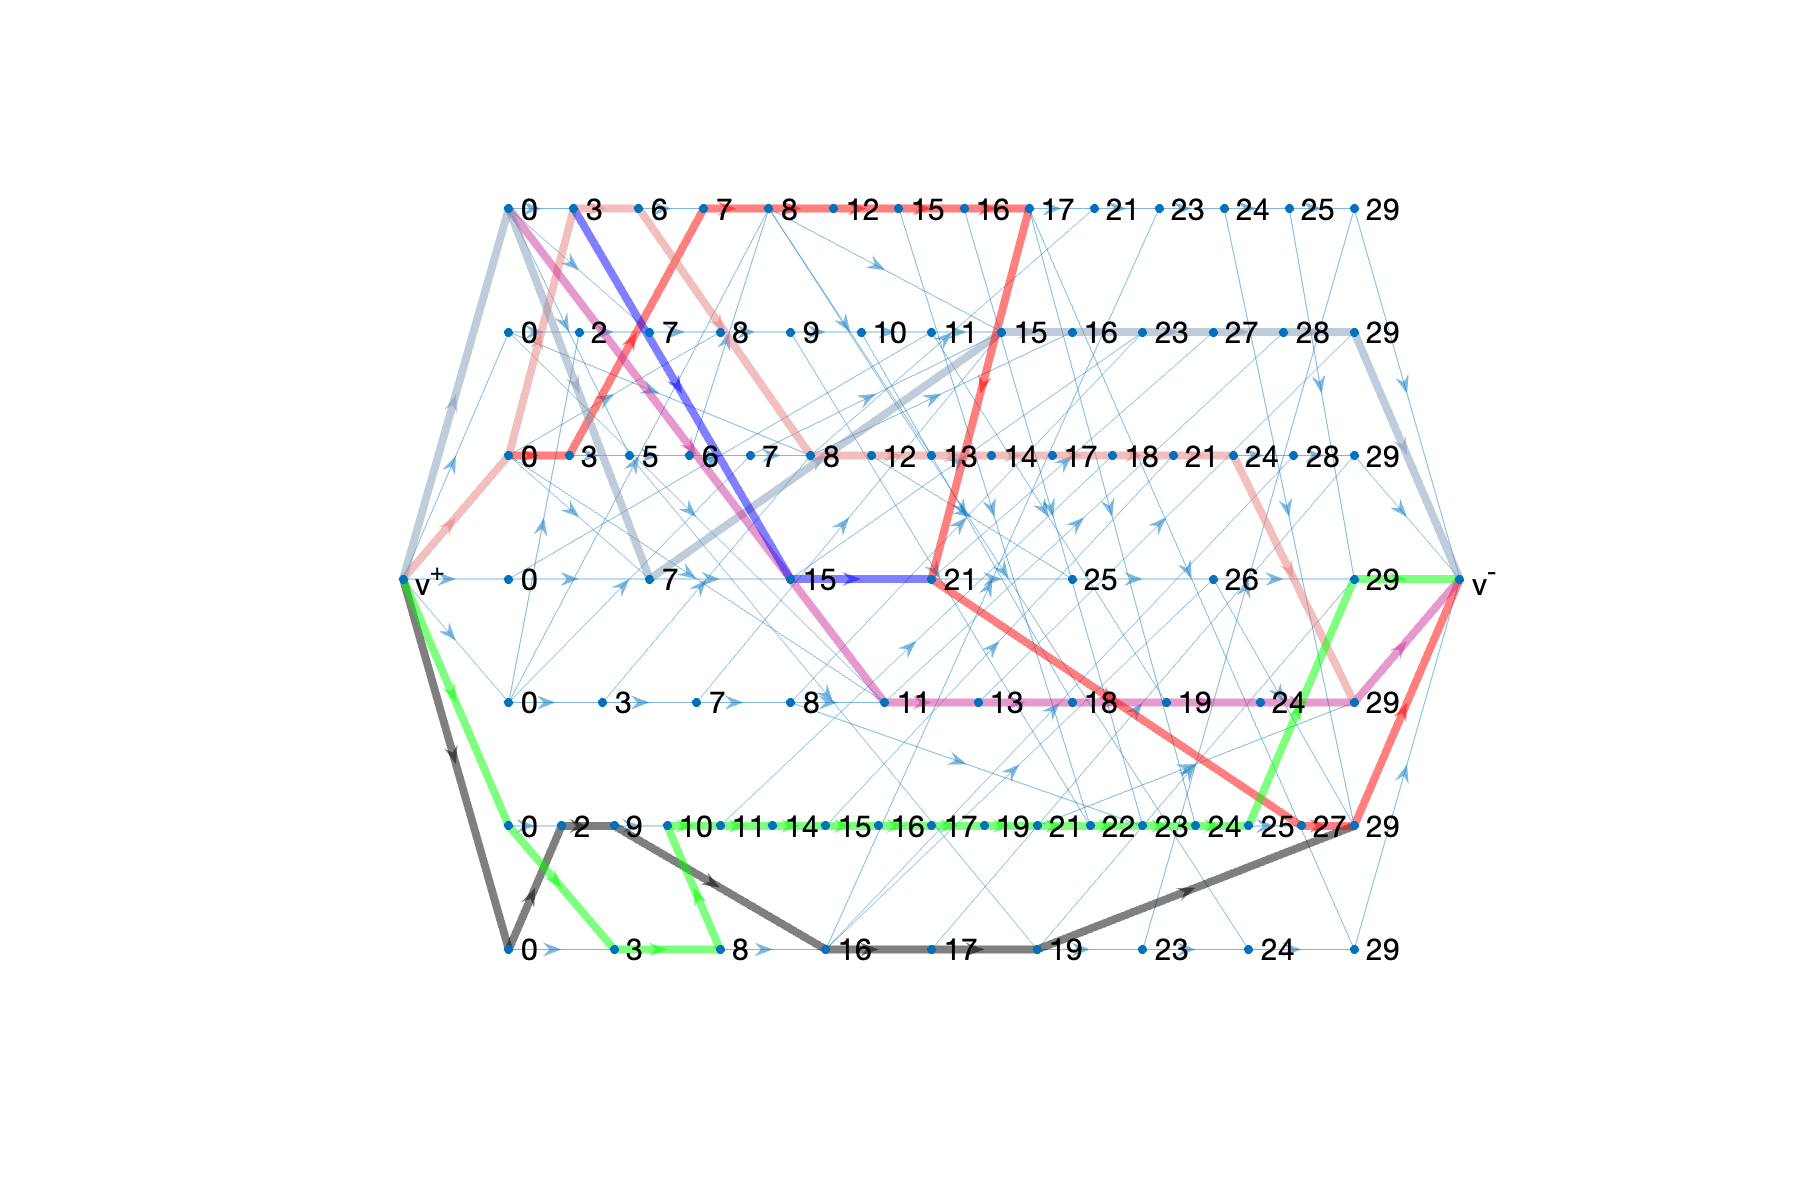
\includegraphics[width=0.47\linewidth,trim = 4cm 0cm 4cm 0cm, clip,valign=c]{7-team-graph.png}}
	\caption{\new{(\ref{fig:Result-plan}) Cross-trajectory co-observation result of a 4 sub-teams task. (\ref{fig:Result-plan-7-team}) Cross-trajectory co-observation result of a 7 sub-teams task.}}\label{fig:Cross-trajectory-result}
  \end{figure}
\vspace{0.2cm}

\begin{cmt}{}{}
	The author assumes “Zone 1” is tolerable and Zone 2 and 3 are hard
constraints, but what if the environment is the opposite? Do you get
infeasible solution? It is very skeptical that the author is making
deliberate assumptions to make the example work in a special case.
\re We acknowledge the limitation of the method proposed in Section II, as it relies on the specific setup, and a safe solution is not always guaranteed to exist. This limitation is explicitly discussed in the manuscript. The chosen result is deliberate, not to make the example work in a special case, but to illustrate that even when APMAPF finds a solution in the grid world, such a plan may fail to guarantee security when transformed into the continuous domain, requiring further manual adjustments. In the revised version, we have further emphasized these limitations and the challenges they aim to address in the simulation results.
Corre
\end{cmt}
\vspace{0.1cm}
\rv
\renewcommand\thesubsection{H}
\subsection{Secured planning results and limitation}\label{sec:ADMM-simulation}
We employ the \new{attack-proof MAPF(APMAPF)} solver [2] on an 8 by 8 grid world with a similar setup to generate a MAPF plan with a co-observation schedule in a grid-world application (Fig.4a). This result is transformed to a continuous configuration space and serves as the initial trajectory input for the ADMM solver with an additional task function targeting the map exploration task. Co-observation schedules are set up using the APMAPF algorithm for two forbidden regions. Reachability constraints are added to ensure an empty intersection between all robots' reachability regions during co-observations and the forbidden regions. {\news It is important to emphasize that an APMAPF solution does not guarantee existence, nor does it ensure a successful transition to the continuous configuration space. In this case, while an APMAPF solution may be found, the secured, attack-proof solution becomes infeasible in the continuous setting because the robots' mobility is no longer restricted to adjacent grids. Additional security measures, such as stationary security cameras or surveillance robots, need to be incorporated. For instance, in this scenario, we deploy a security camera as additional security measure to observe agent 3 at time $8$ to ensure security.}

The simulation result, shown in Fig.4b, displays reachability regions as black ellipsoids, demonstrating empty intersections with Zones 2 and 3. Explicit constraints between reachability regions and obstacles are not activated, assuming basic obstacle avoidance capabilities in robots. The intersections between obstacles and ellipsoids, as observed between agent 3 and Zone 1, are deemed tolerable. All constraints are satisfied, and agents have effectively spread across the map for optimal exploration tasks.

1) Limitations:
Our solution demonstrates the potential of planning with reachability and co-observation to enhance the security of multi-agent systems. {\news However, two primary challenges need to be addressed. Firstly, achieving a co-observation and reachability-secured plan is not always feasible, particularly when obstacles or restricted regions separate the robots, preventing them from establishing co-observation schedules or finding reachability-secured paths. For example, agent 3 in~Fig.4b requires additional security measures to create secured reachability areas. Secondly, security requirements can impact overall system performance, as illustrated by the comparison between~Fig.2b and Fig.4b. The introduction of security constraints resulted in the top left corner remaining unexplored by any robots. This trade-off between security and system performance is particularly significant as system performance is a key factor in the decision of multi-agent system deployments. These challenges are further addressed in Section III, ensuring the effective integration of reachability and co-observation in securing multi-agent systems.}

\begin{cmt}{}{}
	p 8 - A heuristic approach is provided (Algorithm 1); Is it
	almost impossible for the reader to decipher this algorithm without any
	explanations in words.
\re	We have replaced the algorithm with a more detailed and understandable word-based explanation to improve readability and make the approach easier to follow.
\end{cmt}
\rv {\news We begin by adding the start and end locations $(q_{p}(t_0),t_0)$, $(q_{p}(t_2),t_2)$ to $V_{p}$, with $t_{0}=0$, $t_2=T$ as \emph{start} and \emph{end verticies}. Then, we search for the largest $t_{1} \in \{t_{0}+1, \dots ,t_{2}\}$ such that the reachability ellipsoid between $q_{p}(t_{0})$ and $q_{p}(t_{1})$ has no overlap with any of the forbidden areas, i.e. $\mathcal{E}(q_{p}(t_{0}),q_{p}(t_{1}), t_{0},t_{1})\intersect F = \emptyset$. Then $(q_{p}(t_{1}),t_1)$ is added to $V_{p}$. Simultaneously, we search backward to find $q_{p}(t_{3})$ with the smallest $t_{3}\in \{t_{1},\dots,t_{2}-1\} $ that meets the reachability requirement $\mathcal{E}(q_{p}(t_{2}),q_{p}(t_{3}),t_{2},t_{3}) \intersect F = \emptyset$. Then $(q_{p}(t_{3}),t_3)$ is added to $V_{p}$. Finally, we set $t_{0}\leftarrow t_{1}$, $t_{2}\leftarrow t_{3}$ and repeat the same process. The search is stopped when $\mathcal{E}(q_{p}(t_{0}),q_{p}(t_{2}),t_{0},t_{2}) \intersect F = \emptyset$ or $t_{0}>t_{2}$. A toy example is shown in \cref{fig:checkpoint-generate}. }

\begin{cmt}{}{}
	Similar to the comment above, it will be good to introduce what the
“network multi-flow problem” is.
\re 
We have add additional content to introduce the what the "network multi-flow problem" in our setup.
\end{cmt}
\rv \new{We assume that the planned trajectory for each sub-team has a robot operating on it. The co-observation planning problem is then transformed into a network multi-flow problem by modeling the additional robots as flows traveling through $G$. These flows either follow the planned trajectory via trajectory edges $E_t$ or switch teams via cross-trajectory edges $E_c$ to ensure valid and secured paths. Additionally, they are required to visit every checkpoint $V_p$ to meet the security requirements introduced in~\ref{rmk:checkpoints}. This formulation reduces the co-observation problem to finding valid flow patterns in $G$. The problem is then formulated into linear objectives and constraints, enabling the use of Mixed-Integer Linear Programming (MILP) techniques to efficiently compute feasible solutions. }

\begin{cmt}{}{}
	p3 - “rotation derived from a modifie version of Householder
transformations [25].” ; At least a brief introduction of
Householder transformations (in words) must be included for readers who
are not familiar with it.
\re A brief introduction of Householder transformation is added.
\end{cmt}
\rv \new{the rotation matrix $R=H(\nu_\cF(q_1,q_2),\nu_\cE)$ is a \emph{Householder rotation} $H$ (a differentiable linear transformation describing the minimal rotation between the two vectors, see Appendix B for details).}

\begin{cmt}{}{}
This reachability ellipsoid is an over approximation of the exact
reachability region in Definition 3.”; A proof or at least a
reference to the proof should be provided.
\re While we believe that a formal proof is not necessary for this context, we have added additional content to make the approximation more intuitive. This includes a clearer explanation of how the reachability ellipsoid relates to the exact reachability region. These additions aim to enhance the reader's understanding without requiring formal proof.
\end{cmt}
\rv {\news
\begin{definition}\label{sec:ellipsoidal definition}
Consider a robot $i$ starting from $q_{1}$ at time $t_1$ and reaching $q_{2}$ at time $t_2$. The \emph{reachability region} between $t_1$ and $t_2$ is defined as the set of points $q'$ in the free configuration space for which there exists a kinematically feasible trajectory containing $q'$.
\end{definition}

For simplicity, in this paper we consider only a maximum velocity constraint $v_{max}$; the reachability region for $q'$ can then be over-approximated by the following (the over-approximation is obtained by neglecting physical obstacles):
\begin{definition}\label{def:Reachability}
	The \emph{reachability ellipsoid $\cE$} is defined as the region $\mathcal{E}(q_1,q_2,t_{1},t_{2})=\{\tilde{q}\in\mathbb{R}^n: d(q_1,\tilde{q})+d(\tilde{q},q_2)<2a\}$, where $a=\frac{v_{max}}{2}(t_2-t_1)$.
\end{definition}
This region is an ellipsoid because it represents the set of points $q'$ whose sum of distances two \emph{foci} $q_1$ and $q_2$ is less than $2a$, where a is the major radius of the ellipsoid. }
\begin{cmt}{}{}
	Other grammar related comments.
	\re We have carefully reviewed and corrected all listed grammar mistakes, as well as others that were not explicitly mentioned. 
\end{cmt}
%%%%%%%%%%%%%%%%%%%%%%%%%%%%% Rewiewer 2
\newpage
\section{Response to reviewer 2}

%%%%%%%%%%%%% Comment 2.1
\begin{cmt}{}{}

Comments 2.1

\end{cmt}
\vspace{0.1cm}
\noindent
\underline{\textbf{Response:}}
\vspace{0.2cm}

Your Response 2.1

\vspace{0.3cm}


%%%%%%%%%%%%% Comment 2.2
\begin{cmt}{}{}

Comments 2.2

\end{cmt}
\vspace{0.1cm}
\noindent
\underline{\textbf{Response:}}
\vspace{0.2cm}

Your Response 2.2

\vspace{0.3cm}


%%%%%%%%%%%%% Comment 2.3
\begin{cmt}{}{}

Comments 2.3

\end{cmt}
\vspace{0.1cm}
\noindent
\underline{\textbf{Response:}}
\vspace{0.2cm}

Your Response 2.3

\vspace{0.3cm}


%%%%%%%%%%%%% Comment 2.4
\begin{cmt}{}{}

Comments 2.4

\end{cmt}
\vspace{0.1cm}
\noindent
\underline{\textbf{Response:}}
\vspace{0.2cm}

Your Response 2.4

\vspace{0.3cm}


\end{document}